\PassOptionsToPackage{table}{xcolor}
\let\CleanVersionCalendarYear\year
\documentclass{ieeeaccess}
\let\year\CleanVersionCalendarYear

% --- 基础宏包 ---
\usepackage{cite}
\usepackage{amsmath,amssymb,amsfonts}
\usepackage{graphicx}
\usepackage{textcomp}
\usepackage{needspace}

% --- 从你的 header.tex 整合的宏包 ---
\usepackage{lipsum}
\usepackage{tikz}
\usepackage{enumitem}
\usepackage{ragged2e}
\usepackage{listings}
\usepackage{booktabs}
\usepackage{boldline}
\usepackage{pifont}
\newcommand{\xmark}{\ding{53}}
\usepackage{capt-of}
\usepackage[colorinlistoftodos]{todonotes}
\usepackage{multirow}
\usepackage{makecell}
\usepackage{soul}
\usepackage{xcolor}
\usepackage[most]{tcolorbox}
\usepackage{setspace}
\usepackage{xurl} % 允许在 URL 的任何位置断行
\usepackage{tikz}
\usetikzlibrary{positioning, arrows.meta, shapes.arrows}
\usepackage{pgf-pie} % 必须添加这个宏包才能识别 \pie 命令
\usepackage[table]{xcolor} % Add to preamble
\newcommand{\my}[1]{{\color{blue}MY: #1}}
% --- 关键：配置标题颜色为蓝色 ---
\usepackage{caption}
% 手动定义 IEEE Access 的标准蓝色（如果 cls 文件没定义）
\definecolor{accessblue}{RGB}{0,103,165}
% 按照你找到的方法，强制设置标题字体和颜色
\captionsetup{
    font={sf,small,stretch=0.80},
    labelfont={bf,color=accessblue},
    justification=centering
}

% --- 其他自定义样式 ---
\def\BibTeX{{\rm B\kern-.05em{\sc i\kern-.025em b}\kern-.08em
    T\kern-.1667em\lower.7ex\hbox{E}\kern-.125emX}}

\newenvironment{myitemize}%
  {\begin{itemize}[leftmargin=0cm,itemindent=.3cm,labelwidth=\itemindent,listparindent=\parindent,labelsep=0pt,parsep=0pt,topsep=1pt,itemsep=2pt,align=left]}%
  {\end{itemize}}

\newenvironment{myenumerate}%
  {\begin{enumerate}[leftmargin=0cm,itemindent=.5cm,labelwidth=\itemindent,listparindent=\parindent,labelsep=0pt,parsep=1pt,topsep=1pt,itemsep=3pt,align=left]}%
  {\end{enumerate}}

% --- 重新定义颜色 ---
\definecolor{commentgrey}{gray}{0.4}
\definecolor{queryblue}{RGB}{0,103,165}

% --- 极其稳健的样式定义 ---
\lstdefinestyle{elegantQueries}{
    basicstyle=\ttfamily\scriptsize, % 缩小字号防止单栏溢出
    breaklines=true,                 % 自动换行
    columns=fullflexible,
    frame=single,                    % 使用单线框
    rulecolor=\color{gray!30},       % 使用浅灰色边框，不要背景色
    commentstyle=\color{commentgrey}\itshape,
    keywordstyle=\color{queryblue}\bfseries,
    captionpos=b,                    % 标题在下方
    xleftmargin=10pt,                % 增加左边距，防止超出栏宽
    xrightmargin=5pt,
    aboveskip=15pt,
    belowskip=15pt
}

\definecolor{frenzyorange}{RGB}{249, 158, 26}
\newcommand*\circled[1]{\tikz[baseline=(char.base)]{\node[shape=circle,fill=frenzyorange,draw,text=white,inner sep=1pt] (char) {#1};}}
\definecolor{mengxcolor}{RGB}{211, 82, 229}
\newcommand{\lwg}[1]{\textcolor{mengxcolor}{~lwg: #1~}}
\newcommand{\zmy}[1]{{\color{teal}[ZMY: #1]}}
\newcommand\note[1]{#1}

% \definecolor{mygreen}{RGB}{0,128,0}
% \newcommand{\smy}[1]{{\color{mygreen}[SMY: #1]}}
\newif\ifshowrevisions
% Set to \showrevisionsfalse for the clean submission manuscript.
\showrevisionstrue
\soulregister\cite7
\soulregister\ref7
\soulregister\url7
\soulregister\S0
\DeclareRobustCommand{\revise}[1]{\ifshowrevisions{\sethlcolor{yellow}\hl{#1}}\else#1\fi}
\DeclareRobustCommand{\smy}[1]{\revise{#1}}
\DeclareRobustCommand{\revcite}[1]{\ifshowrevisions\begingroup\setlength{\fboxsep}{0pt}\colorbox{yellow}{\cite{#1}}\endgroup\else\cite{#1}\fi}
% November 6 literature update: light blue; earlier revisions remain yellow.
\definecolor{literatureblue}{RGB}{210,235,255}
\DeclareRobustCommand{\revisenew}[1]{\ifshowrevisions{\sethlcolor{literatureblue}\hl{#1}}\else#1\fi}
\DeclareRobustCommand{\newrevcite}[1]{\ifshowrevisions\begingroup\setlength{\fboxsep}{0pt}\colorbox{literatureblue}{\cite{#1}}\endgroup\else\cite{#1}\fi}
\definecolor{revisiongreen}{RGB}{215,245,215}
\DeclareRobustCommand{\revisegreen}[1]{\ifshowrevisions{\sethlcolor{revisiongreen}\hl{#1}}\else#1\fi}
\definecolor{revisionpurple}{RGB}{235,220,250}
\DeclareRobustCommand{\revisepurple}[1]{\ifshowrevisions{\sethlcolor{revisionpurple}\hl{#1}}\else#1\fi}

% ---------------------------------------------------------

\begin{document}

\history{Date of publication xxxx 00, 0000, date of current version xxxx 00, 0000.}
\doi{10.1109/ACCESS.2017.DOI}

\title{\revise{LLM-Assisted OS Security: A Component-Based Scoping Survey}}

\author{\uppercase{Pengchao Yao}\authorrefmark{1,*},
\uppercase{Changhua Sun}\authorrefmark{1},
\uppercase{Xin Sun}\authorrefmark{1},
\uppercase{Bang Lv}\authorrefmark{1},
\uppercase{Yilei Wang}\authorrefmark{1},
\uppercase{Yifeng Wang}\authorrefmark{1},
\uppercase{Yining Mao}\authorrefmark{1},
}

\address[1]{State Grid Zhejiang Electric Power Co., Ltd. Research Institute, Hangzhou, China (e-mails: pcyao@zju.edu.cn, sun\_changhua@zj.sgcc.com.cn, sun\_xin@zj.sgcc.com.cn, lv\_bang@zj.sgcc.com.cn, wang\_yilei@zj.sgcc.com.cn, wang\_yifeng@zj.sgcc.com.cn, mao\_yining@zj.sgcc.com.cn)}
\tfootnote{This work was supported by State Grid Zhejiang Electric Power Co., Ltd. under Project No. B311DS25Z001.}

\markboth
{Yao \headeretal: LLM-Assisted OS Security: A Component-Based Scoping Survey}
{Yao \headeretal: LLM-Assisted OS Security: A Component-Based Scoping Survey}

\corresp{Corresponding author: Pengchao Yao (e-mail: pcyao@zju.edu.cn).}

\begin{abstract}
Operating systems concentrate security-critical complexity: large privileged codebases, 
deep hardware coupling, pervasive concurrency, and decades of compatibility. 
In this setting, large language models (LLMs) are beginning to reshape how we find, 
understand, and remediate vulnerabilities---not by replacing program analyses, fuzzers, or verification, 
but by acting as semantic integrators that connect heterogeneous artifacts
 (\revise{code, specifications, logs/traces, and tool outputs}) and as tool-oriented agents
  that iteratively generate candidate tests, specifications, and patches under deterministic feedback.
\revise{This survey synthesizes research through an OS-centric,
component-based taxonomy spanning kernels, device drivers, networking stacks, file systems, 
privileged system services, and hypervisors/TEEs. We distinguish evaluated LLM-assisted 
OS-security applications from potentially transferable methods and adjacent work that protects LLM systems.} We distill recurring design patterns and their limits, emphasizing a central requirement for deployment: LLM outputs must be treated as candidates, grounded in \revise{verifiable} evidence, and paired with guardrails and reviewable artifacts to preserve correctness, compatibility, and performance. Finally, we outline open challenges---from evidence-grounded evaluation and cross-component reasoning to reviewer-capacity bottlenecks under ``vibe coding''---and identify research directions that prioritize auditable, tool-grounded, and review-scalable LLM assistance \revise{for OS security.}



\end{abstract}

\begin{keywords}
Large Language Models, Operating Systems, Security, Survey
\end{keywords}


\titlepgskip=-15pt

\maketitle

%\input{sections/todo}
%Operating systems concentrate security-critical complexity: large privileged codebases, 
deep hardware coupling, pervasive concurrency, and decades of compatibility. 
In this setting, large language models (LLMs) are beginning to reshape how we find, 
understand, and remediate vulnerabilities---not by replacing program analyses, fuzzers, or verification, 
but by acting as semantic integrators that connect heterogeneous artifacts
 (\revise{code, specifications, logs/traces, and tool outputs}) and as tool-oriented agents
  that iteratively generate candidate tests, specifications, and patches under deterministic feedback.
\revise{This survey synthesizes research through an OS-centric,
component-based taxonomy spanning kernels, device drivers, networking stacks, file systems, 
privileged system services, and hypervisors/TEEs. We distinguish evaluated LLM-assisted 
OS-security applications from potentially transferable methods and adjacent work that protects LLM systems.} We distill recurring design patterns and their limits, emphasizing a central requirement for deployment: LLM outputs must be treated as candidates, grounded in \revise{verifiable} evidence, and paired with guardrails and reviewable artifacts to preserve correctness, compatibility, and performance. Finally, we outline open challenges---from evidence-grounded evaluation and cross-component reasoning to reviewer-capacity bottlenecks under ``vibe coding''---and identify research directions that prioritize auditable, tool-grounded, and review-scalable LLM assistance \revise{for OS security.}



\section{Introduction}

\revise{Operating systems (OSes) underpin modern computing devices---from servers and cloud platforms to mobile phones, IoT devices, and embedded controllers---by multiplexing hardware resources and enforcing trust boundaries between applications, data, and devices. As a result, OS safety and security remain central concerns: a kernel or privileged-service compromise can undermine system availability, confidentiality, or integrity}~\revcite{anderson1972computer}.

\revise{Yet, OSes are difficult to secure. They are implemented largely in low-level systems languages (e.g., C/C++) and evolve into large codebases with long-lived interfaces, hardware coupling, concurrency, and cross-subsystem dependencies}~\revcite{chen2011linux}.
In practice, many real-world attacks are enabled by memory-unsafety and the difficulty of maintaining low-level invariants at trust boundaries; Szekeres \emph{et al.} characterize this as an ``eternal war'' between exploitation and defenses\cite{szekeres13}. Beyond the kernel core, bugs persist in other OS-critical components (e.g., Linux file systems evolving over time\cite{luAAL14}), and even correct isolation can be undermined by policy and configuration complexity (e.g., system-wide mediation in MAC frameworks such as Flask/SELinux\cite{spencer99flask,loscocco01selinux}).

To this end, the community has developed a broad spectrum of toolboxes.
Unfortunately, each technique still faces OS-specific limitations.
\revise{For instance, kernel static analysis can surface many candidate warnings that still require expert triage: DR. CHECKER reported 3,973 flaws at 78\% precision across nine mobile kernels, while studies of Linux-kernel developer responses find that false positives reduce willingness to triage later reports}~\revcite{machiry2017dr,guo2009linux};
\textbf{fuzzing} has been highly effective in practice\cite{boehme16}, and kernel-specific systems further leverage virtualization and hardware support (e.g., kAFL)\cite{kafl17}, but reaching deep kernel states still suffers from the reachability gap and from the difficulty of generating semantically valid, stateful inputs;
\textbf{symbolic execution} can systematically explore corner cases (e.g., KLEE, S2E)\cite{cadar2008klee,chipounov2011s2e}, yet scaling it to OS kernels is challenging due to path explosion, environment modeling (devices, timing, concurrency), and the cost of maintaining accurate models across fast-evolving subsystems;
\textbf{formal methods} can provide high-assurance guarantees, but they remain expensive to apply at scale; recent work such as Selene and AutoRocq highlights that proof engineering and specification effort are still key adoption barriers\cite{zhang2024selene,tu2025agentic}.

The above limitations motivate complementary approaches that reduce the human burden in interpreting tool evidence, reconstructing intent, and validating fixes in fast-evolving OS code.

Large language models (LLMs) have recently emerged as such a complement. 
Built on the Transformer architecture~\revcite{vaswani17}, \revise{modern LLMs show code-related capabilities on benchmarks such as Codex/HumanEval and AlphaCode}~\revcite{chen2021evaluating,li22alphacode}. \revise{GPT-3 demonstrates few-shot in-context learning on evaluated tasks}~\revcite{brown20}, \revise{while compute-optimal scaling work studies the relationship between model size, training data, and compute}~\revcite{hoffmann22}. \revise{Separately, instruction tuning with human feedback improves instruction following in evaluated settings}~\revcite{ouyang22}.


In fact, a growing line of research integrates LLMs into \emph{program analysis} workflows, using models as semantic helpers that translate between code, natural language, and analysis artifacts.
\revise{Common patterns include (i) using LLM guidance to refine static analysis of Linux-kernel UBI code, as in LLIFT}~\revcite{li2024enhancing}, \revise{(ii) translating informal security-protocol descriptions into models for formal verification}~\revcite{mao2025llm}, \revise{and (iii) coupling candidate patch generation with build and reproducer feedback, as in kAgent (previously circulated as CrashFixer)}~\revcite{mathai2025crashfixer}.
\revise{These workflows combine model-generated candidates with analyzers, compilers, or provers that provide checkable feedback.}
\revise{Potential uses in OS-security workflows include summarizing call chains, relating crash traces or static-analysis warnings to code context, and inspecting policy artifacts such as access-control rules; their reliability must be established for each target task.}

\revise{Prior surveys provide complementary perspectives on LLMs in software engineering, vulnerability detection, program repair, and cybersecurity}~\revcite{hou2024large,sheng2025llms,yang2025survey,jaffal25}. \revise{Table~\ref{tab:survey-comparison} compares their primary organizing perspectives with ours. Our contribution is a synthesis organized by OS components and privileged interfaces: it connects each component's security tasks with the artifacts used to validate model outputs, and distinguishes demonstrated OS-security applications from transferable methods and work that protects LLM execution.}

\begin{table*}[t]
\centering
\caption{\revise{Positioning this survey alongside representative prior reviews.}}
\label{tab:survey-comparison}
\footnotesize
\begin{tabular}{@{}p{0.16\textwidth}p{0.33\textwidth}p{0.43\textwidth}@{}}
\hline
\textbf{\revise{Review}} & \textbf{\revise{Primary focus}} & \textbf{\revise{Organizing perspective}} \\ \hline
\revise{Hou et al.}~\revcite{hou2024large} & \revise{LLMs across software-engineering tasks} & \revise{Model use, data, optimization, evaluation and SE tasks} \\
\revise{Sheng et al.}~\revcite{sheng2025llms} & \revise{LLM-based vulnerability detection} & \revise{Detection methods, datasets, evaluation and challenges} \\
\revise{Yang et al.}~\revcite{yang2025survey} & \revise{LLM-based automated program repair} & \revise{Repair paradigms and benchmark evaluation} \\
\revise{Jaffal et al.}~\revcite{jaffal25} & \revise{Cybersecurity applications and LLM threats} & \revise{Security domains, attacks on LLMs and defenses} \\
\textbf{\revise{This survey}} & \revise{LLM assistance for OS security} & \revise{OS components and interfaces, security workflows, validation evidence, and adjacent work} \\ \hline
\end{tabular}
\end{table*}

\revise{We conduct a retrospective survey of selected research on how LLMs have been used, and might be used, to support OS security. We assembled a literature collection through targeted bibliographic searches, as described in Section III.}
We organize this literature by a component-based taxonomy, i.e., \revise{kernel (including syscalls and eBPF), device drivers}, networking, file systems, \revise{privileged user-space system services}, and virtualization/TEEs;
such taxonomy highlights where untrusted inputs enter an OS and what artifacts can ground LLM outputs (e.g., a synthesized eBPF program, a fuzzed driver).

\paragraph*{\textbf{Contributions}} 
\revise{Based on the literature selection and synthesis described in Section III, we make three contributions:}
\begin{itemize}
  \item \textbf{A component-based taxonomy for LLM-assisted OS security.} 
  We organize the design space by major OS components and interfaces, clarifying how threat surfaces, ground-truth artifacts, and evaluation signals differ across subsystems (\S\ref{sec:methodology}).

  \item \textbf{\revise{A synthesis of LLM-assisted OS-security research.}}
  \revise{We summarize selected approaches involving program analysis, synthesis, and fuzzing, distinguishing demonstrated applications to OS security from potentially transferable techniques and adjacent work protecting LLM systems} (\S\ref{sec:os}).
  % designs that close the loop with deterministic feedback (builds, tests, traces, proofs) to make LLM assistance auditable.
  
  \item \textbf{Open problems and future directions.} 
  We identify the most pressing bottlenecks that currently limit practical impact (e.g., evidence grounding and reproducibility). 
  Crucially, we shed light on how \textit{review capacity} \revise{may become} a first-class constraint under high-throughput ``vibe coding'', and we therefore prioritize directions that use LLMs to assist \textit{reviewing} so that LLM assistance scales human governance rather than overwhelming it (\S\ref{sec:future}).
\end{itemize}

\section{Background}
\subsection{OS Security Primer}
\label{sec:bkgd:os}

\revise{An operating system mediates access by processes, users and services to files, devices and other resources. Compromise can undermine confidentiality, integrity and availability; Stuxnet illustrates the potential for disruption of industrial processes}~\revcite{baezner2017stuxnet}. \revise{Foundational work on reference monitors, Multics and protection systems motivates least privilege, complete mediation and isolation}~\revcite{anderson1972computer,corbato1965introduction,lampson1974protection,saltzer1975protection}. \revise{Modern networking, drivers, virtualization and accelerators introduce interconnected trust boundaries and motivate layered defenses.}

\paragraph{\textbf{System calls as the key attack surface}}
Most OSes enforce privilege separation by running applications in an unprivileged mode while centralizing sensitive operations in the kernel, i.e., the separation between user/kernel mode. User space requests privileged operations (e.g., file I/O, process management, and networking) through \textit{system calls}, a standardized interface that transfers control to the kernel.

Because system calls are the main gateway from \textit{untrusted} applications into privileged kernel code, they constitute a primary attack surface. 
Attacks range from passing malformed or adversarial arguments including crafted buffers, filesystem images, and packets, to exploiting unexpected call sequences that trigger corner cases across subsystems, e.g., file systems, IPC, networking, device drivers, BPF/JITs, and virtualization backends, leading to denial-of-service, information disclosure, privilege escalation, or full kernel compromise~\cite{chen2011linux}.

% The ``reference monitor'' concept provides an organizing abstraction: every security-relevant access should be checked by a tamper-resistant mechanism whose complexity is small enough to be analyzable\cite{saltzer75,lampson71}. In practice, faithfully approximating a reference monitor is difficult because the effective policy surface is spread across numerous subsystems, each with subtle notions of identity and authority. Modern implementations thus rely on layered mediation---e.g., discretionary permissions, capability-style privilege separation, and system call filtering/sandboxing---but these layers must track evolving kernel ABIs and cross-subsystem object lifecycles, which creates opportunities for confused-deputy behavior and policy bypasses.

\paragraph{\textbf{Memory bugs as a dominant attack vector}}
\revise{Memory unsafety is a recurring source of OS vulnerabilities, alongside the difficulty of maintaining low-level invariants in concurrent, performance-critical code.}~\revcite{chen2020koobe,xu2015collision,wu2025flow,szekeres13}
\revise{Violations at system-call, packet or driver interfaces can yield out-of-bounds accesses, use-after-free or information disclosure; these primitives may be composed to corrupt security state or gain code execution}~\revcite{chen2020koobe,xu2015collision,wu2025flow,szekeres13}.

\paragraph{\textbf{Defense by isolation: processes, containers, and virtual machines}}
In response to the above attacks and to mitigate them, an OS adopts various \textit{isolation} mechanisms and implements them at multiple layers, each introducing new trust boundaries and failure modes, which can characterized by the following:
\begin{myitemize}
  \item  
  \textbf{Processes} provide an address-space boundary (often reinforced by W$\oplus$X and ASLR), but they still share a kernel, so kernel compromise breaks the isolation model. 
  
  \item 
  \textbf{OS-level virtualization} (i.e., namespaces and cgroups) underpins containers by virtualizing resource views and constraining resource consumption; however, containers typically treat the host kernel as trusted and are therefore sensitive to kernel vulnerabilities and configuration errors (e.g., overly broad capabilities). 

  \item 
  \textbf{Hypervisor-based} virtualization adds an additional privilege layer, with the hypervisor mediating guest access to hardware and exposing a carefully defined virtual device surface. 
  Popek and Goldberg formalize requirements under which an architecture can support efficient virtualization, motivating the modern separation of guest OSs from a smaller virtual machine monitor\cite{popek1974formal}.
  \revise{Vulnerabilities in virtual-device implementations can allow guest-to-host escapes, as demonstrated in attacks on VMware virtual machines}~\revcite{zhao2019breaking}.



\end{myitemize} 



\paragraph{\textbf{Mandatory access control (MAC) and policy-driven mediation}}


Isolation controls \emph{who shares what}, whereas access control governs \emph{who may do what}: OSes mediate operations on objects (files, sockets, devices, processes) based on identities, capabilities, and policy. 
Traditional discretionary access control (DAC) provides owner-centric rules, but it is often complemented by stronger, system-wide mechanisms such as mandatory access control (MAC), which enforces global policies even on privileged services (e.g., restricting networking, module loading, or introspection) and is widely deployed via architectures such as the Flask security server in SELinux\cite{spencer99flask,loscocco01selinux}.

In practice, access control becomes difficult for two reasons. 
First, policy is complex: administrators must reason about large rule sets, defaults, and policy composition, and misconfigurations can silently overgrant or break intended invariants. 
Second, enforcement logic is subtle: correct mediation depends on comprehensive labeling, consistent object identity across subsystems, and correct placement of checks; omissions or inconsistent interpretations lead to logic bugs that allow unintended access despite an apparently sound policy~\cite{lu2019detecting, zhang2019pex}.

\begin{comment}
\paragraph{\textbf{Trusted boot, measured boot, and attestation across the boot chain}}
\note{to decide whether we will keep them}
OS security depends on the integrity of the boot chain, which has become a first-class trust boundary as platforms increasingly rely on complex firmware stacks (UEFI, option ROMs, management engines) and late-loaded components. ``Secure boot'' aims to prevent unauthorized components from executing, while ``measured boot'' records cryptographic measurements that enable attestation against an expected configuration (typically using TPM PCRs)\cite{tpm2spec}. 
These mechanisms extend the reference-monitor mindset earlier in time: rather than mediating accesses at runtime, they attempt to constrain what code is allowed to become part of the trusted computing base. Yet, empirical analyses show that real-world firmware and boot implementations can violate expected measurement properties and that scale and diversity complicate validation; BootKeeper exemplifies how tooling is needed to verify integrity properties over large firmware corpora\cite{bootkeeper19}.
\end{comment}

\paragraph{\textbf{Trusted execution environments (TEEs) as an inverted trust boundary}}
At last, modern OS security \revise{involves} TEEs, which aim to protect sensitive computations even if the OS or hypervisor is compromised, by isolating code and data in hardware-enforced enclaves~\cite{costan2017secure} or secure worlds~\cite{li2019research, Alves2004TrustZoneI}.
This model effectively inverts a classic trust assumption: the OS is no longer the root of trust for application confidentiality/integrity, but instead becomes part of the threat. 
% Intel SGX has been analyzed in depth by Costan and Devadas\cite{costan16sgx}, while TrustZone-based designs demonstrate how TEEs can shield applications from an untrusted commodity OS\cite{guan17trustshadow}. 
\revise{TEEs still depend on carefully designed boundaries. SGX enclaves rely on host-provided services and remain subject to microarchitectural side-channel attacks; these protections therefore apply under specific threat models and do not remove the need to validate enclave--OS interactions}~\revcite{costan2017secure,Cloosters2020TeeRexDA}.
% \my{Slightly change some paragraph A-F, add the leckage}
% \begin{figure}[H]
%   \centering
%   \includegraphics[width=0.7\linewidth]{figures/Transformer_arch.png}
%   \caption{Transformer architecture.~\cite{vaswani17}}
%   \label{fig:transformer}
% \end{figure}
% IEEE Access中放置图片的方法

% \my{Insert Transformer figure and manually adjust position, origional: figure is in the middle of paragraph-f}

\subsection{Large Language Models for Security}
% \subsection{LLMs and Tool-Augmented/Agentic Systems}





In this survey, we use ``LLM'' to refer to large Transformer-based models trained on massive corpora with self-supervised objectives (e.g., next-token prediction).
Due to the multi-head self-attention, Transformer enables efficient parallel training and strong sequence modeling for LLMs~\cite{vaswani17}; 
its architecture is shown in Figure~\ref{fig:transformer}.

% Commonly known as the \textit{scaling law}~\cite{kaplan2020scaling}, LLM's reasoning capability empirically scales with model size, data, and compute.
\smy{Language-modeling loss exhibits empirical scaling relationships with model size, dataset size, and training compute~\cite{kaplan2020scaling}.}
% As a result, a LLM yields strong generalization and in-context learning (few-shot prompting) without task-specific gradient updates~\cite{brown20}. 
\smy{Separately, GPT-3 demonstrates in-context learning on evaluated tasks using few-shot prompts without task-specific gradient updates~\cite{brown20}.} 
\revise{Hoffmann et al. show that compute-optimal training scales data alongside model parameters, changing how a fixed compute budget should be allocated}~\revcite{hoffmann22}.
\revise{Code-generation benchmarks evaluate function-level correctness (Codex/HumanEval) and competitive-programming performance (AlphaCode)}~\revcite{chen2021evaluating,li22alphacode}.


\begin{figure}[htbp]
  \centering
  \includegraphics[width=0.9\linewidth]{figures/transformer.pdf}
  \caption{Transformer architecture}
  \label{fig:transformer}
\end{figure}

\revise{Studies have explored LLM assistance for interpreting code-analysis warnings, translating protocol requirements into formal models, and synthesizing network access-control policies. These results are task-specific and motivate evaluation of similar methods for OS security}~\revcite{wen2024automatically,mao2025llm,mondal2025llm}.
When coupled with deterministic tools (static analyzers, fuzzers, debuggers, CI/test runners), LLMs can help connect heterogeneous evidence into an auditable workflow, while final judgments remain grounded in reproducible tool outputs.

\section{Survey Methodology}
\label{sec:methodology}
\revise{This retrospective literature survey examines LLM-assisted security analysis, testing, verification, and repair across OS components, emphasizing approaches that ground their outputs in verifiable artifacts. Studies that protect LLM-based systems are discussed as adjacent work where relevant, rather than as direct evidence of improved OS security. The collected literature is not claimed to result from a complete, reproducible systematic search.}

\revise{For transparency, we use the search-reporting items of PRISMA-S}~\revcite{rethlefsen2021prismas} \revise{and the selection-reporting guidance of PRISMA 2020}~\revcite{page2021prisma} \revise{to document the available evidence and remaining gaps; referring to these guidelines does not imply that all their items have been satisfied.}

\paragraph{\textbf{Search strategy and venues}}
\revise{The original collection combined targeted searches and foundational references. The 18 surviving historical query formulations are in \url{reproduct/search/}; their database-specific forms, execution dates and results are not established. One formulation combines LLM, large language model or Transformer with operating system security or OS security. TEE and hardware-isolation terms occur, but coverage of neighboring VMM, hypercall, enclave-interface and secure-monitor terms is not established. Representative publication outlets include ICSE, USENIX Security, IEEE S\&P, ASPLOS, OSDI, NeurIPS and ICLR; these are outlets, not verified search databases. Preprints were also considered.}

\revise{On November 5, 2026, an exploratory update used Crossref after automated Google Scholar requests were blocked. It submitted 100 queries with a 2022-01-01 lower publication-date limit and retained up to 20 ranked results per query. Crossref received transformed free-text expressions, not the original Boolean queries. The queries, times, returned counts and status are recorded in \url{reproduct/search/search_metadata.csv}. This later update does not reconstruct the historical search.}

\revise{A separate audit on the same date saved up to 100 results for each of the 100 Crossref queries and for 12 arXiv queries. Crossref and arXiv used different query syntax and date limits; all Crossref queries and two arXiv queries were truncated. Exact DOI and arXiv-identifier matching grouped the 10,467 retrieved rows into 6,408 provisional records. The two truncated arXiv searches were subsequently paginated; their additional records and the time and ranking limitations are documented separately. These bounded searches are exploratory, and their results are not a verified replacement for the historical synthesis. Query logs, linkage rules and scripts are documented under \url{reproduct/search_protocol/} and \url{reproduct/arxiv_pagination/}; the research archive also retains provider responses.}

\revise{The audit records received preliminary triage of titles and available abstracts using \texttt{deepseek/deepseek-flash} via OpenCode. A separate call using the same model assessed the 2,311 records with available abstracts in the 6,408-record snapshot. These model outputs are not independent human screening or final eligibility decisions. Missing abstracts, mismatched evidence excerpts, disagreements and flagged OS-related records remain for review; a check of cited work found a potential model false exclusion. The screening protocol, decision fields, conservative rules and audit are documented under \url{reproduct/screening/} and \url{reproduct/audit/}; individual model inputs and responses are retained in the research archive.}

\revise{The associated search records, screening materials, inventories and supporting scripts are organized in the accompanying \texttt{reproduct/} directory. The exact contents of any public release depend on the materials made available with that release.}

\revise{The stated publication window for candidate research is 2020--2026; older foundational references are used for background rather than as evidence of recent LLM-assisted OS-security methods. Coverage in 2026 is limited to the collected records, not the entire calendar year. For the historical collection, the available materials do not establish exact search dates, a database-specific query log, or a consistent rule for choosing between first-publication and final-publication dates. The venues listed above identify publication outlets rather than a verified list of searched databases. These documentation gaps limit reproducibility and the completeness of the review.}


\paragraph{\textbf{Deduplication and publication versions}}
\revise{The following version-handling principles guide interpretation of the literature; the available spreadsheet does not document a completed record-to-study reconciliation.}
\revise{Version reconciliation requires matching DOI or arXiv identifiers and comparing normalized titles and author metadata; ambiguous or renamed records require comparison of the underlying studies. A preprint and its published counterpart should be treated as one study when they report the same contribution, with the published version preferred when available within the search period. Preprint-only work can be considered under the same substantive criteria, with its publication status identified. Distinct contributions in extended versions require explicit justification before separate counting. These principles do not imply that the 220 scored records already represent 220 unique studies.}

\paragraph{\textbf{Eligibility and screening}}
\revise{The criteria below define the intended scope of the core synthesis, rather than certifying the eligibility of every previously scored entry.}
For the core synthesis, a study must (i) fall within the stated date and document-type limits; (ii) use an LLM as a substantive part of a security analysis, testing, repair, or verification method; (iii) explicitly target an OS component or privileged interface; and (iv) provide sufficient methodological detail and evaluation evidence to assess that OS-security application. Evidence may include experiments, case studies, or formal results; public artifact availability is recorded rather than assumed to be mandatory.
Excluded from the core synthesis are duplicates, out-of-window studies, non-LLM methods, generic code-generation or application-security studies without an explicit OS target, and opinion or promotional material without assessable research evidence. Work that uses OS isolation or TEEs solely to protect LLM execution is treated as adjacent research rather than direct evidence that LLMs improve OS security. Surveys, foundational papers, standards, and vendor documentation may support background discussion but are not counted as independent core studies.
\revise{In particular, ERP, OA, and mail studies confined to application business logic or message-content analysis are excluded from the core synthesis.}
\revise{The surviving materials do not provide a complete record-level log of title/abstract decisions, full-text exclusions, or retrieval failures, nor do they establish whether language or full-text availability restrictions were applied consistently. Eligibility criteria describe the intended scope and do not certify a final eligible-study set.}

\paragraph{\textbf{\revise{Relevance scoring and evidence}}}
\revise{The exploratory update returned 2,000 Crossref result rows across the 100 queries. DOI-based merging yielded 1,454 candidate records; records without a DOI were kept separately. A ranked subset of 200 was inspected rapidly using titles and available abstracts, and 101 entries were selected as direct or adjacent candidates. Six matched previously retained records and 95 were added as new rows. The resulting inventory contains 130 retained legacy rows and 95 new rows, totaling 225. Earlier low-relevance records were not systematically carried forward. These are candidate records, not a census of unique eligible studies. Matching used recorded identifiers or normalized titles where available; unresolved duplicates and preprint/publication versions can remain. The candidate-origin labels are provisional and should not be equated with final eligibility decisions.}

\revise{The later assessment assigns topical relevance scores of 0 (no substantive connection), 1 (background), 2 (adjacent or transferable) and 3 (direct OS-security candidate). The 225 records contain 1, 37, 164 and 23 entries at these scores, respectively. Scores indicate topical fit rather than study quality or verified eligibility; the inventory records whether judgments used abstracts, accessible conclusions or earlier notes.}

\paragraph{\textbf{\revise{Screening personnel and limitations}}}
\revise{The surviving historical records do not document who screened each stage, independent duplicate screening or disagreement resolution. The later update does not establish independent human adjudication either. Inter-rater agreement cannot be reconstructed, and decisions near the core/adjacent boundary may be subjective.}

\paragraph{\textbf{\revise{Record counts and provenance}}}
\revise{Table~\ref{tab:selection-counts} distinguishes the historical scored-record inventory from the later merged candidate inventory. The archived historical file has 485 records, of which 220 carry scores 1--3: 45, 116 and 59 respectively. These counts match those in the earlier manuscript, which designated 59 score-3 records for in-depth review; the exact correspondence to the previously submitted supplementary file cannot be established from counts alone. Neither number is a verified count of unique eligible studies. The remaining 265 rows include scores of zero and missing or other values; they cannot be interpreted as documented exclusions. The later inventory draws on a different selection and updated ratings, so its totals cannot replace the historical numbers in a single sequential screening flow. A record-level crosswalk and unresolved matches are provided with the supplementary inventory.}

\begin{table}[htbp]
\centering
\caption{\revise{Available literature-record counts and their limits.}}
\label{tab:selection-counts}
\small
\begin{tabular}{@{}>{\RaggedRight\arraybackslash}p{0.44\columnwidth}>{\RaggedRight\arraybackslash}p{0.50\columnwidth}@{}}
\hline
\textbf{Quantity} & \textbf{Count/status} \\ \hline
\revise{Original search hits and selection stages} & \revise{Unknown; full search and decision logs unavailable} \\
\revise{Historical scored records} & \revise{220 records; 59 formerly designated for in-depth review} \\
\revise{Updated merged candidate inventory} & \revise{225 records, including 23 provisional score-3 records} \\
\revise{Separate discovery audit} & \revise{6,408 identifier groups; later arXiv pagination produced 1,168 additional unmatched identifiers} \\
\revise{Unique studies after version reconciliation} & \revise{Not established} \\
\revise{Unique eligible studies and final in-depth set} & \revise{Not established} \\ \hline
\end{tabular}
\par\smallskip
\parbox{0.96\columnwidth}{\footnotesize\revise{These counts describe different record sets, not consecutive stages. Preliminary scores do not certify eligibility.}}
\end{table}

\revise{The candidate and historical inventories and their interpretation are provided in \url{reproduct/}. Later-added provider reports are recorded separately in the literature addendum and are not included in those candidate counts. The accompanying Crossref metadata log documents the exploratory update; it does not reconstruct the earlier search. A separate citation-level audit maps manuscript references to the candidate and search records where identifiers or source-checked aliases permit; unmatched citations include background, adjacent work and unresolved cases, and are not automatically counted as omissions. Version aliases and source-supported corrections are retained with their evidence under \url{reproduct/audit/}, and the revised manuscript's citation mapping is in \url{reproduct/revision/}. Table~\ref{tab:llm-kernel-related} illustrates representative core and related work rather than a complete eligibility record. The KernelGPT workflow in the device-driver discussion is a literature-based illustration, not an experiment performed to validate the survey framework (\S~\ref{sec:os:driver}).}

\begin{table*}[t]
\caption{\revise{Representative works and their underlying techniques.}}
\label{tab:llm-kernel-related}
\centering
\footnotesize
\begin{tabular}{>{\RaggedRight\arraybackslash}p{0.22\textwidth}>{\RaggedRight\arraybackslash}p{0.72\textwidth}}
\hline
\textbf{\revise{Technique}} & \textbf{\revise{Representative work}} \\
\hline
\revise{Analysis and fuzzing} & \revise{KernelGPT refines syscall specifications; RandLuzz directs fuzzing on evaluated programs; SyzAgent guides kernel-test generation. Kernel applicability of RandLuzz requires separate evaluation}~\revcite{yang2025kernelgpt,feng2025fuzzing,syzagent25}. \\
\hline
\revise{Formal verification} & \revise{Selene studies seL4 proof generation, while AutoRocq and FVEL use prover feedback to refine proof attempts}~\revcite{zhang2024selene,tu2025agentic,lin2024fvel}. \\
\hline
\revise{Synthesis} & \revise{KNighter and Kgent generate checkers and eBPF extensions. QLCoder met its vulnerable-versus-patched detection criterion for 53.4\% of 176 CVEs across 111 Java projects; its applicability to kernel code requires separate evaluation}~\revcite{yang2025knighter,zheng2024kgent,wang2025qlcoder}. \\
\hline
\revise{Patching and repair} & \revise{kAgent and SAN2PATCH generate candidate repairs, while PortGPT targets kernel patch backporting; candidates require target-specific validation}~\revcite{mathai2025crashfixer,kim2025logs,li2025portgpt}. \\
\hline
\end{tabular}
\end{table*}

\section{LLMs for OS Security}
\label{sec:os}

\subsection{Overview and taxonomy}


\begin{figure}[t]
  \centering

  % Resizebox ensures it fits exactly into one column width
\resizebox{\columnwidth}{!}{
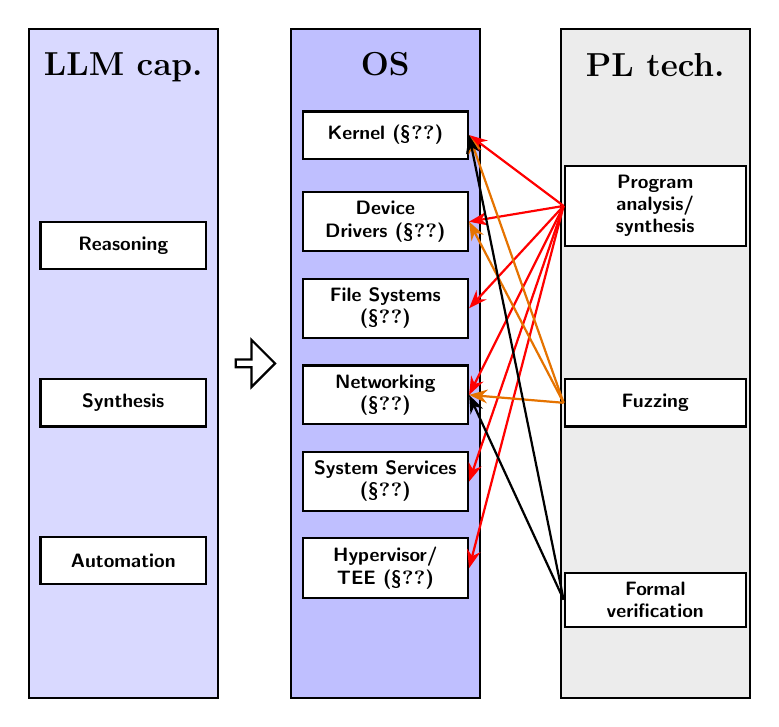
\begin{tikzpicture}[
    font=\sffamily\bfseries,
    % Narrower containers for column fit
    container/.style={draw, fill=#1, minimum width=2.4cm, minimum height=8.5cm, thick},
    % Smaller item boxes
    itembox/.style={draw, fill=white, minimum width=2.1cm, minimum height=0.6cm, 
                    align=center, thick, font=\sffamily\scriptsize\bfseries},
    % Arrow styles
    redarrow/.style={-Stealth, red, line width=0.8pt},
    goldarrow/.style={-Stealth, orange!90!black, line width=0.8pt},
    blackarrow/.style={-Stealth, black, line width=0.8pt}
]

    % --- Column 1: LLM cap. ---
    \node[container=blue!15] (LLM) {};
    \node[anchor=north, font=\large, yshift=-0.2cm] at (LLM.north) {\textbf{LLM cap.}};
    
    \node[itembox, yshift=1.5cm] (Reasoning) at (LLM.center) {Reasoning};
    \node[itembox, yshift=-0.5cm] (Synthesis) at (LLM.center) {Synthesis};
    \node[itembox, yshift=-2.5cm] (Automation) at (LLM.center) {Automation};

    % --- The Large Block Arrow ---
    \node[single arrow, draw, minimum height=0.5cm, minimum width=0.6cm, 
          right=0.2cm of LLM, anchor=west, inner sep=1pt, thick] (BlockArrow) {};

    % --- Column 2: OS ---
    \node[container=blue!25, right=0.9cm of LLM] (OS) {};
    \node[anchor=north, font=\large, yshift=-0.2cm] at (OS.north) {\textbf{OS}};

    % Positioned carefully to avoid "OS" title overlap
    \node[itembox, yshift=2.9cm] (Kernel) at (OS.center) {Kernel (\S\ref{sec:os:kernel})};
    \node[itembox, yshift=1.8cm] (Drivers) at (OS.center) {Device\\Drivers (\S\ref{sec:os:driver})};
    \node[itembox, yshift=0.7cm] (FileSys) at (OS.center) {File Systems \\(\S\ref{sec:os:fs})};
    \node[itembox, yshift=-0.4cm] (Networking) at (OS.center) {Networking \\(\S\ref{sec:os:network})};
  
    \node[itembox, yshift=-1.5cm] (Services) at (OS.center) {System Services \\(\S\ref{sec:os:services})};
    \node[itembox, yshift=-2.6cm] (Hypervisor) at (OS.center) {Hypervisor/\\TEE (\S\ref{sec:os:tee})};

    % --- Column 3: PL tech. ---
    \node[container=gray!15, right=1.0cm of OS] (PL) {};
    \node[anchor=north, font=\large, yshift=-0.2cm] at (PL.north) {\textbf{PL tech.}};

    \node[itembox, yshift=2.0cm, minimum width=2.3cm] (ProgAnal) at (PL.center) {Program\\analysis/\\synthesis};
    \node[itembox, yshift=-0.5cm, minimum width=2.3cm] (Fuzzing) at (PL.center) {Fuzzing};
    \node[itembox, yshift=-3.0cm, minimum width=2.3cm] (Formal) at (PL.center) {Formal\\verification};

    % --- Connections ---
    % Red arrows
    \foreach \dest in {Kernel, Drivers, Networking, FileSys, Services, Hypervisor}
        \draw[redarrow] (ProgAnal.west) -- (\dest.east);

    % Gold arrows
    \foreach \dest in {Kernel, Drivers, Networking}
        \draw[goldarrow] (Fuzzing.west) -- (\dest.east);

    % Black arrows
    \foreach \dest in {Kernel, Networking}
        \draw[blackarrow] (Formal.west) -- (\dest.east);

\end{tikzpicture}
}
  \caption{The structure of this survey, showing how fundamental LLM capabilities benefit OS security and the underpinning programming language techniques.}
  \label{fig:llm-os-mindmap}
\end{figure}

% An OS concentrates security-critical complexity: large privileged codebases, deep hardware interaction, concurrency, and decades of backwards compatibility \cite{bessey2010few}. These factors make vulnerabilities as well as logic bugs hard to prevent and expensive to triage for an OS, as signals are noisy and scattered across code, specifications, and tool outputs \cite{guo2009linux}. For instance, static analysis and address sanitizers are known hard for an OS kernel~\cite{guo2009linux,serebryany2012addresssanitizer} and to produce many false alarms~\cite{guo2009linux,wen2024automatically}.
An OS concentrates security-critical complexity: large privileged codebases, deep hardware interaction, concurrency, and decades of backwards compatibility~\cite{bessey2010few}. These factors make vulnerabilities and logic bugs hard to prevent and expensive to triage, as signals are noisy and scattered across code, specifications, and tool outputs~\cite{guo2009linux,wen2024automatically}. Static-analysis reports can require substantial triage effort, whereas AddressSanitizer detects memory errors dynamically~\cite{guo2009linux,wen2024automatically,serebryany2012addresssanitizer}.

\revise{LLMs offer a complementary way to interpret and connect these artifacts. Evaluations of code-trained models demonstrate useful code-generation capabilities, motivating their use as assistants rather than as independent correctness oracles}~\cite{chen2021evaluating}.
For example, in static-analysis-based bug finding, an LLM can summarize long call chains, explain data-structure/locking assumptions, and help validate whether an alarm is plausible by cross-checking code context and constraints~\cite{wen2024automatically}.

% while the final decision should still rely on deterministic evidence (e.g., reproducing inputs, traces, and tests).

\paragraph{Taxonomy of this survey}
\revisegreen{We organize the literature by OS component and interface, and compare studies within and across components according to the security workflows they support. The component dimension identifies the interfaces and execution environments under study, while the workflow dimension identifies the LLM's task, the artifacts it produces, and how those artifacts are evaluated.} The following sections describe their security tasks, supporting tools, and evaluation evidence.
\begin{itemize}
  \item \textbf{Kernel.} The kernel is the core of an OS. Here, we cover process and memory management, scheduling, page management, and syscall subsystems. We also consider eBPF, which permits restricted user-provided programs to execute in kernel context subject to verifier and permission checks.
  \item \textbf{Device drivers.} Drivers bridge privileged kernel code and hardware through interfaces such as \texttt{ioctl}. Their analysis must account for device-specific state and the OS and hardware environment.
  \item \textbf{Networking.} The OS networking stack processes and routes packets while maintaining stateful protocol logic, with data flowing through shared structures such as \texttt{sk\_buff}.
  \item \textbf{File systems.} File systems map files and directories onto storage devices, manage metadata such as names and permissions, and provide buffering and caching. Journaling and copy-on-write designs support crash consistency and recovery.
  \item \textbf{System services.} These user-space components often run with elevated privileges and provide logging and auditing, service management, update and configuration functions, and process orchestration. In this survey, the category covers privileged OS services.
  \item \textbf{Hypervisors and TEEs.} Hypervisors virtualize hardware for guest operating systems. TEEs provide hardware-enforced isolation for code and data. We treat both as kernel-adjacent components because their interfaces shape system trust boundaries.
\end{itemize}

\paragraph{Survey organization}
%We first provide an overview of OS security challenges and motivate why LLMs are a useful ``assistant'' for connecting heterogeneous evidence (code, documentation, static-analysis warnings, sanitizer traces, and fuzzer crashes). 
Following our component-based taxonomy (Figure~\ref{fig:os-arch}), we list the representative techniques in Table~\ref{tab:llm-kernel-related}, and describe how LLMs benefit each component: kernel (\S~\ref{sec:os:kernel}), device drivers (\S~\ref{sec:os:driver}), file systems (\S~\ref{sec:os:fs}), networking (\S~\ref{sec:os:network}), TEEs (\S~\ref{sec:os:tee}) and privileged user-space system services (\S~\ref{sec:os:services}). 
For each component, we highlight the security challenges, typical techniques/defenses, artifacts, and evaluation used in that component. 
Finally, we summarize cross-cutting themes (e.g., grounding, feedback loops, and validation) and discuss open problems and future research directions.

\revise{Table~\ref{tab:representative-evidence} compares representative studies, their evaluations, and the limits of their reported evidence.}
% Sources for numerical claims (publication snapshots, not live counts):
% KernelGPT ASPLOS 2025 abstract and Table 3: https://yangchenyuan.github.io/files/ASPLOS25-KernelGPT.pdf
% SyzAgent FASE 2025, Sec. 4 and Table 1: https://arxiv.org/pdf/2503.02301
% BugLens ASE 2025, abstract and Table I: https://www.cs.ucr.edu/~zhiyunq/pub/ase25_buglens.pdf
% KNighter SOSP 2025, Sec. 5 and Table 2: https://yangchenyuan.github.io/files/SOSP25-KNighter.pdf
% MigGPT NeurIPS 2025, Sec. 6.1 and Table 5: https://proceedings.neurips.cc/paper_files/paper/2025/file/3760dbb5835bf0b771c3f83cb27ef2c0-Paper-Conference.pdf
% PathSentinel arXiv:2407.11279, Sec. VII-D: https://arxiv.org/html/2407.11279
\begin{table*}[t]
\centering
\caption{\revise{Representative LLM-assisted OS security approaches and their reported evaluations.}}
\label{tab:representative-evidence}
\begingroup
\setlength{\tabcolsep}{2pt}
\footnotesize
\begin{tabular}{@{}>{\RaggedRight\arraybackslash}p{0.105\textwidth}>{\RaggedRight\arraybackslash}p{0.14\textwidth}>{\RaggedRight\arraybackslash}p{0.15\textwidth}>{\RaggedRight\arraybackslash}p{0.15\textwidth}>{\RaggedRight\arraybackslash}p{0.17\textwidth}>{\RaggedRight\arraybackslash}p{0.18\textwidth}@{}}
\hline
\revise{Study} & \revise{OS target and task} & \revise{LLM role and validation} & \revise{Evaluation and baseline} & \revise{Reported result} & \revise{Scope and limitation} \\
\hline
\revise{KernelGPT}~\revcite{yang2025kernelgpt} &
\revise{Linux drivers and sockets; syscall fuzzing} &
\revise{Generates and repairs Syzkaller specifications using validation feedback} &
\revise{Kernel fuzzing; Syzkaller and SyzDescribe baselines} &
\revise{24 new bugs; 11 CVEs and 12 fixes reported in the ASPLOS paper} &
\revise{Findings depend on inferred interfaces and execution coverage; accepted specifications need not be complete.} \\
\hline
\revise{SyzAgent}~\revcite{syzagent25} &
\revise{Linux kernel; directed fuzzing} &
\revise{Guides Syzkaller test generation and mutation during fuzzing} &
\revise{27 target-function cases; Syzkaller baseline; three two-hour runs per case} &
\revise{18 of 27 cases had at least 10\% relative improvement under the paper's $\omega$ metric} &
\revise{Preliminary target-reachability evaluation; the hit-rate metric is not a vulnerability count.} \\
\hline
\revise{BugLens}~\revcite{li2025towards} &
\revise{Linux kernel drivers; taint-style warning triage} &
\revise{Reasons over analyzer reports, impact and source-code constraints} &
\revise{Android Linux 4.14.150 driver reports; Suture and CodeQL-SOD} &
\revise{Suture-report precision rose from 0.10 to 0.72; four real bugs previously dismissed as false positives in Suture's manual review} &
\revise{Refines existing reports and depends on the input analyzer's dataflow; reported gains are dataset-specific.} \\
\hline
\revise{KNighter}~\revcite{yang2025knighter} &
\revise{Linux kernel; static bug-pattern detection} &
\revise{Synthesizes and refines checkers from historical bug-fix patches} &
\revise{61 bug-fix patches; generated checkers applied to the kernel} &
\revise{92 new bugs, including 77 confirmed and 30 CVEs, in the SOSP paper} &
\revise{Checker construction depends on input patches; the 32.2\% false-positive rate applies to reports from the evaluated triage pipeline.} \\
\hline
\revise{MigGPT}~\revcite{dang2025miggpt} &
\revise{Linux kernel; patch migration and security backporting} &
\revise{Retrieves relevant code and generates migrated patches} &
\revise{Out-of-tree migration and FixMorph CVE-backporting benchmark with 350 instances} &
\revise{On CVE backporting, GPT-4-turbo semantic match: 85.43\% baseline vs. 91.78\% with MigGPT} &
\revise{Semantic match is not a proof of patch correctness; outcomes depend on model and target version.} \\
\hline
\revise{PathSentinel} \revcite{lee2024static} &
\revise{Android applications and core services; filesystem-access vulnerabilities} &
\revise{Generates test exploit code using findings from static and access-control analysis} &
\revise{16 path-traversal cases; LLM-generated tests with analysis context} &
\revise{Usable tests for 7 simple and 9 complex cases with appropriate context} &
\revise{The LLM assists validation; vulnerability detection is performed by program and policy analysis.} \\
\hline
\revise{LLM-CAL}~\revcite{gadey2026llmcal} &
\revise{TEE boundary design; annotate cryptographic code for TEE placement} &
\revise{Fine-tuned LLM labels security-sensitive code to support partitioning} &
\revise{4,010 C source files; held-out line-level classification} &
\revise{98.41\% F1 and 97.50\% recall for line-level labels} &
\revise{Code-label metrics do not validate the security of a resulting TEE partition.} \\
\hline
\revise{OpenAI pipeline}~\revcite{openai2026paths} &
\revise{Linux kernel; local privilege escalation} &
\revise{Finds candidates, reproduces bugs, develops exploits and proposes patches} &
\revise{Stock Linux distribution; provider report; human review} &
\revise{1,724 reproduced vulnerabilities; 948 working LPE exploits} &
\revise{Provider-reported results depend on target configuration and resources; patches require review.} \\
\hline
\end{tabular}
\endgroup
\end{table*}

\paragraph{\revise{Cross-study synthesis.}}
\revise{The eight studies intervene at different points in a security workflow. KernelGPT improves the specifications supplied to a fuzzer, while SyzAgent steers mutation toward target functions; BugLens refines reports produced by an analyzer, KNighter generates the analyzer itself, MigGPT proposes migrated patches, PathSentinel assists exploit validation for Android applications, LLM-CAL labels cryptographic code for TEE partitioning, and the OpenAI pipeline reports exploitability assessment and candidate patches. Coverage or target hit rate, report precision, newly confirmed bugs, patch semantic match, code-label metrics and exploit counts measure different outcomes and should not be ranked as if they were a shared benchmark. Improved reachability does not by itself establish a vulnerability, agreement with a reference patch does not establish security correctness, and high code-label scores do not validate a resulting TEE boundary.}

\revise{Tool feedback supplies useful checks, but each study retains a distinct evidence boundary: fuzzing requires executable interfaces and a meaningful oracle; report triage inherits the analyzer's candidate set and dataflow; patch-guided checker synthesis depends on representative historical fixes; and patch migration must preserve the target kernel's semantics. These dependencies motivate reporting baseline configuration, dataset construction, model and kernel versions, false positives, and independent reproduction or review together with success metrics.}


% A key survey observation is that OS components differ along three axes that directly shape LLM utility: (i) \,\emph{where untrusted input enters} (system calls, ioctls, packets, and on-disk images), (ii) \,\emph{what constitutes ground truth} (crash traces, coverage, proofs, differential oracles), and (iii) \,\emph{what the security objective is} (memory safety, isolation, policy compliance, availability). Consequently, effective LLM-based methods tend to be component-aware, combining natural-language reasoning with verifiable evidence and tool feedback.

\begin{figure}[t]
  \centering
  \includegraphics[width=0.8\columnwidth]{figures/arch-crop.pdf}
  \caption{Simplified OS architecture and major kernel subsystems discussed in this survey.
  Note the highlighted components are discussed in this paper.}
  \label{fig:os-arch}
\end{figure}


\subsection{\textbf{Kernel (core services, syscalls, and eBPF)}}
\label{sec:os:kernel}
The kernel is the primary trusted computing base for commodity OS security: as mentioned earlier (\S~\ref{sec:bkgd:os}) it implements core services (e.g., scheduling, memory management, namespace management, IPC) and mediates access to hardware and global resources; 
it mainly exposes the system call layer for apps, where untrusted user-space inputs cross into privileged code, often through long-lived compatibility surfaces such as ABIs, legacy syscalls, and subsystem-specific \texttt{ioctl} and \texttt{netlink}. 
As a result, kernel security work is typically organized around (i) hardening kernel code and auditing syscall-related logic, (ii) constraining privilege and ambient authority inside the kernel, and (iii) maintaining security invariants (e.g., file permissions) under concurrency and performance constraints.

A particularly salient modern subsystem is extended BPF (eBPF), which allows \textit{restricted} user-provided programs to execute in kernel context for observability (i.e., tracing kernel activities), networking, and security enforcement. 
eBPF expands the kernel attack surface beyond traditional syscalls: it introduces a verifier with complex semantic requirements, JIT compilation, helper APIs, and shared maps that connect unprivileged or semi-privileged code to kernel state. 
This creates both opportunities (programmable security mechanisms) and risks (verifier soundness bugs, JIT issues, and subtle capability/permission interactions), making eBPF a natural focus for automated reasoning and testing.

Within the above scope, LLM assistance commonly falls into four categories:
\begin{itemize}
  %\item \textbf{Formally verified kernel}: 
  \item \textbf{Formal verification of kernels}: 
  \revise{Formal verification can establish specified kernel properties under explicit modeling assumptions.}
  Yet, writing specifications as well as theorem proving is time-consuming and tedious.   
  LLMs can assist this process by helping convert informal kernel intent (e.g., API contracts, verifier invariants, lock/refcount discipline) into candidate formal specifications, and to propose proof artifacts (lemmas, tactics, proof scripts) that are accepted or rejected by a proof assistant for validation.
  
  \item \textbf{Kernel program analysis and fuzzing}:
  Kernel program analysis and fuzzing generate high-volume, noisy signals (e.g., static-analysis warnings, sanitizer traces, and fuzzer crashes) that are difficult to triage against a large codebase.
  LLMs can help by summarizing subsystem architecture and long call chains, inferring likely data/control-flow relationships near syscall handlers, and proposing hypotheses that map low-level symptoms to candidate root causes.
  For dynamic testing, LLMs can also generate syscall- and eBPF-centric harnesses, seed programs, and stateful input sequences, and iteratively refine them using tool feedback such as coverage, verifier errors, and crash reports.
  
  \item \textbf{Kernel artifact synthesis}: 
  Kernel relies on security-sensitive auxiliary artifacts to operate, e.g., security configurations, permission lists, and eBPF program templates.
  Yet these artifacts take experienced kernel developers to compose, and can lead to kernel crashes or security breaches if not handled properly.   
  LLMs may help synthesize such artifacts at a low cost -- they translate high-level security intents into kernel configuration/policy snippets, and proposing targeted instrumentation to expose invariants or collect evidence.  
  % synthesized artifacts should be treated as untrusted until validated.
  
  % generating scaffolding code (e.g., syscall exercisers, eBPF program templates, tracing scripts), translating high-level security intent into kernel configuration/policy snippets, and proposing targeted instrumentation to expose invariants or collect evidence; synthesized artifacts should be treated as untrusted until validated.
  
  \item \textbf{Kernel patching and repair}:
  Kernel is rapidly evolving software, which undergoes constant patching and fixes, e.g., for bugs or compatibility.
  Yet, kernel patching/repairing is a high-stakes, multi-step workflow --- localize the root cause, craft a minimal fix consistent with kernel conventions, and demonstrate correctness via builds, tests, and regression reproductions.
  LLMs can help automate parts of this loop by integrating existing patches, proposing candidate patches and commit messages, drafting regression tests/reproducers from crash reports, and iteratively revising the patch in response to deterministic feedback (compiler errors, test failures, sanitizer reports, and fuzz regressions).
\end{itemize}

\paragraph{Formal verification of kernels} \revise{LLM-assisted machine-checked reasoning spans both kernel-specific and transferable work. Selene directly studies project-scale proof generation for seL4; AutoRocq reports evaluations on general verification benchmarks and Linux kernel modules; other autoformalization work proposes candidate statements or proof steps for checking by a prover}~\revcite{zhang2024selene,tu2025agentic,wu2022autoformalization}. \revise{A proof checker can reject invalid proof steps, while the correctness of the formal specification and its correspondence to the intended kernel property remain separate obligations}~\revcite{wu2022autoformalization,yang2023leandojo}.

In this workflow, the LLM proposes lemmas, tactics, proof sketches, or intermediate invariants, while a proof assistant such as Coq or Rocq checks candidate proof steps. The proof-engineering burden remains a key obstacle to wider adoption.

\revise{The following studies provide general or transferable context for kernel verification.}
\revise{VeriBench is a general benchmark for generating Lean~4 verification code from Python programs.}~\revcite{miranda2025veribench}
\revise{GPass is a Coq-based neural theorem prover rather than an LLM system.}~\revcite{chen2025gpass}
\revise{A Unit Proofing Framework proposes a research agenda for code-level verification.}~\revcite{amusuo2025unit}
\revise{ABSINT-AI studies LLM-assisted abstract interpretation for JavaScript property-access errors.}~\revcite{wang2025absint}

\revise{AutoRocq reports general verification evaluations, including Linux kernel modules, while FVEL evaluates an interactive proof environment on general code-verification tasks.}~\revcite{tu2025agentic,lin2024fvel}
\revise{WhiteFox is an LLM-assisted compiler-fuzzing method and is included only as a potentially transferable testing technique.}~\revcite{yang2024whitefox}

\begin{tcolorbox}[colback=gray!8, colframe=gray!55, boxrule=0.4pt, left=1mm, right=1mm, top=0.8mm, bottom=0.8mm, title=Key findings] From a systems-security perspective, these works highlight several recurring challenges: (i) bridging the specification gap between informal kernel intent and formal statements that are both provable and security-meaningful; (ii) scaling proof search and tactic synthesis across rapidly evolving code and configurations; and (iii) maintaining trustworthy toolchains and auditable artifacts (proof scripts, traces, and extracted invariants) in the presence of probabilistic LLM outputs. \end{tcolorbox}

\paragraph{Kernel program analysis and fuzzing} 
\revise{Program analysis and fuzzing are natural entry points for LLM assistance in kernel security because kernel code contains implicit invariants that can be difficult to reconstruct and validate.}

% Recent surveys summarize how LLMs are being integrated into vulnerability detection pipelines and how they interact with classical program-analysis techniques\cite{sheng26survey,mata25survey}.

At a high level, LLM-assisted program analysis typically uses the model to (a) summarize long call chains and cross-subsystem control flow, (b) infer candidate data-structure and locking invariants, (c) triage and post-refine static-analysis alarms, and (d) connect low-level symptoms (e.g., a sanitizer report) to plausible root causes and security impact. 
For kernels, especially the Linux kernel, these capabilities are most useful when the model’s claims are grounded in explicit evidence, e.g., identifying the syscall dispatch path
(e.g., \texttt{do\_syscall\_64} $\rightarrow \cdots \rightarrow$\texttt{\_\_x64\_sys\_*} on x86-64 Linux, with intermediate dispatch functions omitted), 
the relevant task/cred objects (\texttt{task\_struct}, \texttt{cred}), and the concrete data-structure/locking context (\texttt{struct file} / \texttt{inode} / \texttt{dentry}, \texttt{sk\_buff}, RCU, spinlocks, refcounts). 
In triage, an LLM can help connect a report (KASAN/KCSAN stack trace, syzbot repro) to likely lifetime or concurrency mistakes (e.g., missing \texttt{kref\_get}/\texttt{kfree\_rcu}, wrong lock ordering). % but should be cross-checked against compiler types, CFGs, and dynamic traces \note{cite}.

\textbf{Refinement and static-analysis noise reduction.}
A recurring theme is using LLMs to reduce the analyst burden from high-volume static-analysis alarms.
\revise{LLIFT augments static analysis for Linux-kernel use-before-initialization (UBI) detection; the paper reports four previously undiscovered UBI bugs acknowledged by the Linux community}~\revcite{li2024enhancing}.
% In addition, \textbf{KNighter} explores synthesizing executable checkers from natural-language bug-pattern descriptions to scale auditing across large kernel trees\cite{yang2025knighter}.
In addition, \textbf{KNighter} synthesizes executable static-analysis checkers from historical kernel bug-fix patches, with patch-based validation and iterative refinement~\cite{yang2025knighter}.
\revise{BugStone combines LLVM-based program analysis with LLM-guided reasoning for large-scale bug discovery}~\revcite{wu2025one}.

\revise{Together, these approaches illustrate how LLMs can help interpret analysis results or synthesize checks for kernel auditing.}

\textbf{Contextual, kernel-specific detection.}
% Beyond generic alarm refinement, several works apply LLM reasoning to kernel-specific complexity, such as precise dataflow reconstruction (e.g., taint-style detection in \textbf{\textit{Towards More Accurate Static Analysis}})\cite{li2025towards} and concurrency reasoning (e.g., \textbf{\textit{When threads meet interrupts}} for deadlock detection)\cite{ye2024threads}.
\smy{Beyond generic alarm refinement, \textbf{BugLens} uses LLM-guided post-refinement for taint-style bug detection in the Linux kernel~\cite{li2025towards}.}

\revise{Guided Vulnerability Imagination (GVI) augments vulnerability-detection training data with synthesized bug patterns for its evaluated software targets.}~\revcite{yong2025gvi}

Broader dataflow-centric reasoning capabilities have also been explored in general settings (e.g., \textbf{LLMDFA}) and can be adapted to kernel-style code where pointer-rich dataflow, aliasing, and lifetimes across subsystems (VFS, networking, drivers) drive many security-relevant behaviors\cite{wang2024llmdfa}. 
In practice, adapting these methods to the kernel often requires making the analysis ``kernel-aware'' (e.g., modeling common primitives such as refcounts, RCU, and per-CPU data) and grounding outputs in concrete code references.

\revise{More general frameworks such as Fuzz4All study LLM-assisted fuzzing across programming languages and parsers.}~\revcite{xia2024fuzz4all}
% Furthermore, the reasoning capabilities of LLMs have been specialized for directed fuzzing; for instance, \textbf{RandLuzz} ~\cite{feng2025fuzzing} employs LLMs to generate high-quality seeds that satisfy complex path constraints, significantly improving the efficiency of reaching deep target code locations needed by kernel code. 
Furthermore, the reasoning capabilities of LLMs have been specialized for directed fuzzing; for instance, \textbf{RandLuzz} ~\cite{feng2025fuzzing} employs LLMs to generate high-quality seeds that satisfy complex path constraints, \smy{improving targeted exploration in its evaluated programs.} 
\revise{HLPFuzz applies LLM-based constraint solving to language-processor fuzzing}~\revcite{yang2025hybrid}. \revise{These general techniques may inform kernel fuzzing, subject to evaluation on kernel targets.}
% \textbf{Snowplow} further strengthens kernel fuzzing by learning a white-box test mutator that predicts promising argument mutations from the current/desired coverage context\cite{gong2025snowplow}.

Specification- or oracle-driven fuzzing is particularly relevant to kernels, where the key bottleneck is not input generation but deciding whether behavior is incorrect.
eBPF is emblematic: its semantics are constrained by a verifier and by non-trivial safety rules, motivating specification-based oracles for detecting misbehavior.
% \textbf{SpecCheck} is a recent and representative example of this line of work, using an explicit specification-derived oracle to flag semantic misbehavior beyond crash-based signals~\cite{lyu2025ebpf}.
% While it is currently still based on manually devised rules, such approaches align well with LLMs: a model can help draft candidate specifications, generate diverse eBPF programs that explore corner cases, and explain misbehavior reports, while the oracle enforces correctness~\cite{lyu2025ebpf}.
\smy{As non-LLM background on specification-based testing, \textbf{SpecCheck}, part of \textbf{Veritas}, checks eBPF-verifier behavior against a specification-derived oracle~\cite{lyu2025ebpf}.}

\begin{tcolorbox}[colback=gray!8, colframe=gray!55, boxrule=0.4pt, left=1mm, right=1mm, top=0.8mm, bottom=0.8mm, title=Key findings]
\revise{Across the studies reviewed here, LLMs assist with navigating subsystems, proposing hypotheses, and generating structured tests. Correctness and security conclusions still depend on task-specific evidence such as checked proofs, test oracles, traces, and reproduced crashes.}
\end{tcolorbox}

\paragraph{\revisenew{Patch-based vulnerability reproduction}}
\revisenew{K-Repro takes a kernel fix commit as input and constructs a PoC through source inspection, VM execution and debugging. On 100 KernelCTF cases, its primary configuration reproduces 56 cases in the initial run and 64 cumulatively after repeated runs. Its analysis identifies concurrency and object-lifetime constraints as recurring obstacles to reproduction}~\newrevcite{pu2026krepro}.

\revisenew{SyzHarness generates a parameterized harness from the patch and source context, preserves the prerequisite setup logic, and exposes uncertain inputs to Syzkaller mutation. Coverage feedback guides harness refinement. Its evaluation confirms 78 of 100 KernelCTF reproductions by checking failure behavior before and after the corresponding patch and matching the execution evidence to the affected code}~\newrevcite{li2026syzharness}.

\revisenew{These methods allocate the reproduction effort differently: K-Repro iterates over executable PoCs using debugging feedback, whereas SyzHarness separates setup construction from concrete input search. The latter gives the fuzzer a constrained search space while retaining LLM assistance for repairing missing setup steps. Their reported outcomes should be read with the model, search budget and reproduction criterion in Table}~\ref{tab:representative-evidence}.

\paragraph{\revise{Exploitability assessment and exploit development}}
\revise{Recent provider reports extend LLM-assisted kernel analysis to exploitability assessment.} \revisenew{OpenAI reports that its pipeline analyzed 2,308 candidate findings and dynamically reproduced 1,724 in a Linux distribution. It generated 1,169 working local privilege-escalation exploits, corresponding to 948 unique LPE vulnerabilities counted using distinct patches after variant analysis.} \revise{The pipeline generated candidate patches for human review; the reported run cost approximately 1.21 million US dollars in API credits}~\revcite{openai2026paths}.
\revise{Anthropic reports that Claude Mythos Preview constructed Linux local privilege-escalation chains involving multiple vulnerabilities, while other remotely triggerable memory vulnerabilities resisted its exploitation attempts}~\revcite{anthropic2026mythos}.
\revise{These results illustrate both offensive capability and defensive validation for prioritizing fixes. They are provider-reported observations under specific targets and resource budgets; a working exploit demonstrates impact in its tested environment, and a generated patch still requires maintainer review and validation.}

\paragraph{Kernel auxiliary artifact synthesis}
\revise{The kernel-specific synthesis work reviewed here generates auxiliary artifacts, such as static-analysis checkers and eBPF extensions}~\revcite{yang2025knighter,zheng2024kgent}.

% \textbf{Checker synthesis for kernel auditing.} KNighter exemplifies ``analysis checker synthesis'' in which an LLM derives bug patterns from historical kernel bug-fix patches and synthesizes executable static-analysis checkers, enabling scalable auditing of large kernel codebases~\cite{yang2025knighter}. Conceptually, this treats the LLM as a compiler from informal security intent to formalized detection logic; the key technical challenge is constraining the synthesized checker so that it is both sound enough to be useful and precise enough to avoid overwhelming analysts with noise ~\cite{yang2025knighter}.
\textbf{Checker synthesis for kernel auditing.} KNighter exemplifies ``analysis checker synthesis'' in which an LLM derives bug patterns from historical kernel bug-fix patches and synthesizes executable static-analysis checkers, enabling scalable auditing of large kernel codebases~\cite{yang2025knighter}. \smy{Conceptually, this turns patch-derived bug patterns into executable static-analysis checkers;} the key technical challenge is constraining the synthesized checker so that it is both sound enough to be useful and precise enough to avoid overwhelming analysts with noise ~\cite{yang2025knighter}.

% \textbf{Exploit and pathology synthesis for security assessment.}
% Beyond defensive tooling, synthesis techniques are also applied to reconstruct and generate exploits or exploit-enabling program behaviors, including data-oriented exploits that target non-control-flow data structures to bypass modern mitigations. 
% For example, \textbf{Lancet} formalizes the reconstruction of logical paths from crashes to exploit primitives \cite{dai2025lancet}. 
% More broadly, recent work demonstrates sound and efficient exploit synthesis by framing the task as a programming language synthesis problem, where the model must satisfy complex data-flow constraints to produce viable attack payloads ~\cite{bailluet2025nothing}. 
% This application underscores how synthesis can automate the evaluation of kernel resilience against sophisticated data-corruption threats.

\textbf{Kernel extension and monitoring synthesis via eBPF agents.}
The closest setting to ``kernel code synthesis'' arises with safe extension mechanisms such as eBPF ~\cite{zheng2024kgent}. Since eBPF programs can be loaded at runtime (subject to verifier constraints), they provide a constrained substrate where LLMs can synthesize kernel-resident monitoring or enforcement logic without rebuilding the kernel ~\cite{gao2025offloading}.
\revise{Kgent, initially circulated as KEN, illustrates an agentic approach in which an LLM produces and refines eBPF programs for user-specified kernel extension tasks. Its evaluation focuses on program correctness; applying generated extensions to security enforcement requires separate validation}~\revcite{zheng2024kgent}.
% Related systems (e.g., \textbf{AgentSight}) similarly use eBPF as a safe substrate to synthesize kernel-resident monitoring/observability logic \cite{zheng2025agentsight}. 
This line of work highlights the synthesis--verification interplay: eBPF's verifier and helper APIs provide guardrails, but subtle semantic gaps (kernel version differences, helper availability, and non-functional constraints such as overhead) still demand testing and careful operational controls.



\begin{tcolorbox}[colback=gray!8, colframe=gray!55, boxrule=0.4pt, left=1mm, right=1mm, top=0.8mm, bottom=0.8mm, title=Key findings] 

\revise{The evaluated synthesis systems turn bug-fix patterns or user requests into executable checkers or constrained extensions.}
\end{tcolorbox}

\paragraph{Kernel patching and repair}



\revise{Kernel live-update work studies safe application of changes to running systems, while migration and backporting studies evaluate patch adaptation across kernel versions. These tasks make the running system and target version part of the validation context}~\revcite{arnold2009ksplice,dang2025miggpt,li2025portgpt}.
% As a result, LLM-based patching for kernels is increasingly framed as an \emph{agentic} workflow in which the model iteratively proposes edits, consults tool feedback (builds, tests, sanitizers, fuzzers), and revises until a candidate patch is both correct and reviewable \cite{mathai2025crashfixer,nong2025appatch}.
\revise{A representative kernel-repair system, kAgent (formerly CrashFixer), proposes candidate patches for Linux kernel crashes and refines them using build and reproducer feedback}~\revcite{mathai2025crashfixer}.

\revisenew{Live-kBench evaluates kernel crash repair through a continuously updated bug collection and kEnv, a shared environment for building kernels and executing reproducers. Its initial Live-kBench-2512 release contains 534 bugs. It measures crash resolution through repeated execution, root-cause localization through patch overlap, and equivalence to developer fixes through an LLM judge. Separate reporting of these outcomes helps identify whether an agent removes the observed failure and how its changes relate to the developer's repair}~\newrevcite{huang2026livekbench}.

Within the emerging domain of memory-safe kernel development, \textbf{Rust-doctor} \cite{yang2025rust} addresses the unique complexities of the Rust compiler's borrow checker by automating the repair of ownership and lifetime errors through balanced training data and targeted LLM reasoning. Related work explores structured reasoning and iterative refinement for vulnerability repair (e.g., \textbf{LoopRepair}~\cite{looprepair25}), as well as approaches that explicitly decompose repair reasoning into intermediate steps (e.g., tree-of-thought style analysis in \textbf{SAN2PATCH})\cite{kim2025logs}. 
% Prompt- and interaction-centric methods such as \textbf{APPATCH} and \textbf{PatchAgent} emphasize that patch quality often depends as much on the prompting strategy and feedback integration as on raw model capacity, particularly when mimicking developer workflows (hypothesis, edit, test, and explain)\cite{nong2025appatch,xue2025pagent}.
\smy{\textbf{APPATCH} studies LLM-based vulnerability repair~\cite{nong2025appatch}, while \textbf{PAGENT} combines repository-level static analysis with LLM-based type inference to repair type-related errors in patches generated by software-engineering agents~\cite{xue2025pagent}.}

Beyond generating a single fix, several kernel-specific tasks involve reasoning over patch \emph{ecosystems} \cite{dang2025miggpt}. 
Migration and backporting are critical in practice because security fixes must be propagated across versions and vendor trees \cite{dang2025miggpt,li2025portgpt}. 
\textbf{MigGPT} targets migration of out-of-tree Linux kernel patches across versions\cite{dang2025miggpt}, while \textbf{PortGPT} focuses on automated backporting of kernel patches to older stable branches\cite{li2025portgpt}. 
\revise{MigGPT also reports a CVE patch-backporting evaluation, distinct from its broader patch-migration task}~\revcite{dang2025miggpt}.
Finally, ``patch intelligence'' tasks such as stable-patch classification can be used to triage which commits should be backported or prioritized; 
\textbf{PatchScope} exemplifies this direction by providing fine-grained classification of Linux stable patches using LLM enhancement\cite{liu2025patchscope}.


% Finally, LLMs facilitate the assessment of exploitability across complex environments. To manage long-term maintenance, \textbf{AEM} leverages LLMs for cross-version exploitability assessment, determining if a root cause persists across kernel releases despite significant code drift\cite{jiang2023aem}. 
% By anchoring probabilistic model outputs in deterministic evidence, these approaches transform raw crash data into structured security intelligence.


\begin{tcolorbox}[colback=gray!8, colframe=gray!55, boxrule=0.4pt, left=1mm, right=1mm, top=0.8mm, bottom=0.8mm, title=Key findings] 
\revisenew{Kernel repair covers both generating fixes from crash evidence and adapting existing patches across versions. Reproducer execution and comparison with developer fixes assess different aspects of a repair; Live-kBench makes these outcomes and their variation over time available in a shared evaluation environment}~\newrevcite{huang2026livekbench}.
% because they act as semantic integrators over scattered evidence—turning crash reports and sanitizer traces into coherent hypotheses, proposing localized edits, and iteratively improving patch candidates using tool feedback (builds, tests, sanitizers, fuzzers) until the result is reviewable. 
% This “agentic” generate–validate loop aligns well with kernel workflows and helps navigate patch ecosystems (e.g., migration/backporting and stable-patch triage) . 
\end{tcolorbox}


\subsection{\textbf{Device Drivers}}
\label{sec:os:driver}

Device drivers sit at the boundary between kernel software and physical devices.
They mediate stateful interactions under elevated privileges~\cite{swift2003improving}.
\revise{Driver analysis must account for device-specific state, kernel interfaces, and models of the OS and hardware environment; prior work studies these modeling requirements and ioctl-mediated driver testing}~\revcite{ball2006thorough,renzelmann2012symdrive,corina2017difuze}.
% A fundamental challenge underlying these difficulties is the specification--implementation gap.
\revise{Static analysis of drivers requires models of the operating system and device environment; building and maintaining these models is challenging across diverse hardware}~\revcite{ball2006thorough}.
\revise{SymDrive documents path-exploration and environment-modeling challenges for driver analysis, including complex ioctl inputs and interrupt behavior}~\revcite{renzelmann2012symdrive}. \revise{DiFuze takes a complementary approach by using driver-interface information to guide fuzzing}~\revcite{corina2017difuze}.

Recent research explores the use of large language models (LLMs) to augment traditional driver analysis techniques, positioning LLMs as a heuristic bridge when specifications are missing or incomplete.
\revise{These approaches use semantic regularities in source code, documentation, and development artifacts to reduce modeling gaps.}
% This makes careful example--claim alignment especially important in a survey and suggests the area is still emerging.
\revise{The following discussion focuses on driver-facing surfaces, such as \texttt{ioctl}-mediated entry points, and auditing workflows evaluated on kernel device drivers.}

\textbf{\revise{Fuzzing with incomplete specifications.}}
Coverage-guided fuzzers struggle on driver attack surfaces when valid inputs require non-trivial structure and cross-field dependencies.
\revise{KernelGPT addresses part of this challenge.}
It improves Linux kernel fuzzing by using LLMs to automatically synthesize and refine Syzkaller syscall specifications (i.e., syzlang) from implementation artifacts, and to repair these specifications based on validation feedback~\revcite{yang2025kernelgpt}.
This matters for driver security because many driver code paths are exercised through syscall-mediated entry points, especially \texttt{ioctl}, where better specifications can help fuzzers generate well-formed call sequences that reach deeper driver handlers.
% We view this line of work as strengthening the specification layer that fuzzers rely on, not as complete recovery of all driver-specific \texttt{ioctl} semantics.

\paragraph{Literature-based workflow example: KernelGPT}
\revise{KernelGPT's published workflow illustrates how generated specifications are validated and used for fuzzing; this literature-based example is not an independent empirical validation of the survey's taxonomy}~\cite{yang2025kernelgpt}.
\begin{myenumerate}
  \item \textbf{Inputs.} \revise{Kernel implementation artifacts provide evidence about syscall interfaces and the structures needed to exercise kernel and driver code.}
  \item \textbf{LLM-generated artifact.} \revise{The model proposes Syzkaller syscall specifications in syzlang, translating implementation information into inputs usable by the fuzzer.}
  \item \textbf{Validation and refinement.} \revise{Specification-validation feedback guides subsequent corrections, keeping the model's proposals within a tool-checked refinement loop.}
  \item \textbf{Downstream use.} \revise{The resulting specifications support syscall-based fuzzing, including driver-facing entry points. The workflow connects source-level interface information to executable testing artifacts.}
\end{myenumerate}
\revise{The generated specifications and validation feedback should remain inspectable: accepted specifications may omit interface semantics, and failures require reproduction and root-cause analysis before a vulnerability is confirmed.}

\textbf{Static analysis on kernel device drivers.}
LLMs have also been used as post-refinement components that reduce analyst burden without replacing conventional analyzers.
\textbf{BugLens} evaluates on Linux kernel device drivers by taking warnings produced by prior static analyzers and guiding an LLM through structured reasoning to assess security impact and validate constraints against the surrounding code context.
% In this setting, LLMs act as a semantic triage layer that filters spurious reports and highlights actionable cases~\cite{buglens25}.
In this setting, LLMs act as a semantic triage layer that filters spurious reports and highlights actionable cases~\revcite{li2025towards}.
This is useful for driver auditing, where benign low-level idioms and performance-driven patterns can confuse scalable analyses.

% Despite promising results, open challenges remain regarding robustness, scalability, and the trustworthiness of LLM-assisted reasoning in high-privilege kernel code.



% \zmy{After reviewing the relevant literature, only KernelGPT and BugLens address device drivers. Thus, I retain only these two works and highlight that LLM-based research for device driver security remains largely unexplored.}

\begin{tcolorbox}[colback=gray!8, colframe=gray!55, boxrule=0.4pt, left=1mm, right=1mm, top=0.8mm, bottom=0.8mm, title=Key findings]
\revise{The driver-facing studies discussed here use LLMs to synthesize fuzzing specifications for driver-reaching entry points or to refine static-analysis results.}
% Across these categories, LLMs primarily serve as augmentation mechanisms rather than standalone solutions, complementing traditional analyses by compensating for incomplete specifications and high-noise auditing pipelines.
\revise{Additional evaluation on diverse drivers and hardware remains an open research direction.}
% Research on LLM for Device Drivers Security is scarce, making it a field that urgently requires further investigation.
\end{tcolorbox}





\subsection{\textbf{File systems}}
\label{sec:os:fs}

File systems manage on-disk data formats for both efficiency and security. 
\revise{File-system implementations have reported security vulnerabilities across multiple components. Cai et al. analyze 157 CVE cases and characterize their attack procedures, root causes, consequences, and mitigations}~\revcite{cai2019understanding}.
% improving the data locality for various workloads and scenarios, e.g., F2FS specializes hot/cold regions for flash longevity\cite{f2fs}. 
\revise{File-system reasoning also involves invariants across on-disk formats, journaling and recovery logic, and interactions among VFS, block-layer, and page-cache code. These relationships motivate possible LLM assistance.}

\revise{Some recent work studies LLMs for file-system efficiency. STELLAR tunes parameters of parallel file systems for HPC workloads, a task its authors describe as complex and manpower-intensive}~\revcite{egersdoerfer2025stellar}.
% STELLAR achieves human-like efficiency by functioning as an agentic workflow that can read software manuals, analyze I/O trace logs, and execute trial runs on real hardware to refine its strategies.
There are only limited work which directly applies LLMs to file systems for better security, which we next describe in detail.


\revise{The most closely related work is PathSentinel, which analyzes filesystem-access vulnerabilities in Android applications and core services, including path traversal, hijacking, and luring attacks. Static program analysis and access-control analysis identify candidate issues; the LLM is used to generate exploit tests for validation, rather than to detect vulnerabilities or to analyze the filesystem implementation itself}~\revcite{lee2024static}.
% Rigorous testing on Samsung and OnePlus devices running Android 12 and 14 uncovered 51 previously unknown vulnerabilities with an exceptionally high accuracy rate. 
\revise{This work illustrates how program analysis and LLM-assisted exploit generation can support validation of the targeted Android filesystem vulnerabilities.}

\revise{Egersdoerfer et al. investigate ChatGPT-based anomaly detection on parallel-file-system logs in a preliminary study}~\cite{egersdoerfer2023early}.
% Early exploration of using chatgpt for log-based anomaly detection on parallel file systems logs, HPDC'23
\revise{The approach uses summary-based memory to retain context across sequential log windows.}
\revise{It prompts the model for both a status prediction and an explanation, giving administrators additional information to inspect alongside the predicted anomaly.}
\revise{The preliminary evaluation reports promising results against the tested baselines.}

\revise{SysGPT is a fine-tuned model for serial-performance optimization; the paper includes a file and storage systems case study}~\revcite{park2025principles}.
% By transforming performance optimization from an intuition-driven task into a structured process, this work helps developers identify and implement targeted improvements for the sequential bottlenecks that limit overall system speed as well as giving security advice of file systems.
By transforming performance optimization from an intuition-driven task into a structured process, this work helps developers identify and implement targeted improvements for the sequential bottlenecks that limit overall system speed~\cite{park2025principles}.

\revise{SysSpec uses LLMs to turn high-level designs into file-system code and adapts specification principles from formal methods. Its evaluation concerns functional correctness and system evolution, not security properties; applying its approach to security invariants remains an open direction}~\revcite{liu2025sharpen}.

\begin{tcolorbox}[colback=gray!8, colframe=gray!55, boxrule=0.4pt, left=1mm, right=1mm, top=0.8mm, bottom=0.8mm, title=Key findings]
\revise{The file-system work discussed here focuses more on efficiency and operations than on direct security tasks. PathSentinel uses an LLM to assist validation of Android application filesystem-access findings.}
\end{tcolorbox}



\subsection{\textbf{Networking}}
\label{sec:os:network}

\revisenew{An OS network stack processes packets through kernel networking and transport protocols and their packet-buffer abstractions. This section covers testing of Linux socket interfaces and analysis of protocol implementations. KnitFuzz directly exercises kernel networking, while studies such as ChatAFL evaluate application-layer protocols}~\newrevcite{zhang2026knitfuzz,meng24}.

\revise{For stateful protocols, valid message sequences can reach implementation states that malformed inputs do not; application-layer studies such as ChatAFL use state-aware generation to explore these behaviors}~\revcite{meng24}.
\revisenew{LLMs contribute executable socket tests as well as models and grammars derived from protocol specifications.}

\paragraph{RFC-Based Specification Formalization}
Similarly, network stack can also use formal verification for better security;
differently, the formal verification of network stack  must bridge the semantic gap between implementations and external natural-language standards (e.g., RFCs). 
Recent work explores using LLMs to parse RFC prose, extract requirements, and translate them into verification-ready representations.

For instance, \textbf{Mao et al.} targets RFC-derived requirements by converting natural-language specifications into models that can be consumed by protocol verification workflows to check whether intended security properties hold under the modeled assumptions~\cite{mao2025llm}.
By formalizing natural-language requirements into logic-oriented models, such approaches can support more rigorous assessment of whether a protocol design or implementation aligns with its intended security guarantees.

\revise{PARVAL uses a multi-agent framework to extract format specifications from C source and RFC documents, then checks parser inconsistencies in an FRRouting BFD-parser case study}~\revcite{zheng25}.
Similarly, \textbf{CryptoFormalEval} benchmarks the capability of LLMs to translate cryptographic protocol descriptions into formal syntax, such as Tamarin Prover, allowing for automated discovery of logical flaws through interaction with the formal toolchain~\cite{curaba24}.

\paragraph{Protocol State Inference and Fuzzing.}
\revisenew{KnitFuzz targets state dependencies in Linux socket system calls by generating C seed programs with an LLM. It combines selective memory instrumentation for mutation with a state-aware remote endpoint for network interactions. The published abstract reports two kernel bugs, including one previously unknown vulnerability, across its evaluated Linux kernels. KernelGPT supplies a fuzzer with interface descriptions; KnitFuzz supplies executable programs that establish socket-call context}~\newrevcite{zhang2026knitfuzz,yang2025kernelgpt}.

In the domain of fuzzing, LLMs also enhance coverage by helping infer protocol structure (e.g., grammars or state machines) and generating structured message sequences. 
This capability is important because traditional mutation-based fuzzers often fail to synthesize protocol-valid packets required to traverse deep states without prior knowledge of the protocol's grammar and transition constraints. 

\revisenew{Application-layer protocol testing addresses message structure and session state.}
\revise{As a non-LLM comparison, HDHunter uses gray-box generation of structured request/response sequences to expose HTTP desynchronization flaws in parsers and intermediaries}~\revcite{mu2025silent}.
\textbf{ChatAFL} demonstrates this by extracting machine-readable grammars from RFCs to guide state exploration in protocols like RTSP and FTP, and reporting improvements over baseline fuzzing strategies~\cite{meng24}. 
To address undocumented or private protocols, \textbf{LLM-Boofuzz} parses real traffic captures to synthesize executable fuzzing scripts and employs an agentic workflow to iteratively optimize test cases based on runtime feedback~\cite{wang25boofuzz}. 
Furthermore, \textbf{mGPTFuzz} demonstrates scalability by processing over a thousand pages of the Matter IoT specification to construct finite state machines, enabling stateful testing that can reveal non-crash logical vulnerabilities~\cite{ma24}.


\begin{comment}
\note{no notable works. Thus directly omit.}
\paragraph{Intent-Driven Configuration and Synthesis}
Synthesis in networking primarily manifests as Intent-Based Networking (IBN), where systems translate high-level natural-language operational goals into low-level, vendor-specific configurations and policies. 
By allowing operators to specify goals without mastering heterogeneous command-line syntaxes, this abstraction can reduce human-induced misconfigurations which is a common contributor to network-level security incidents.
In this setting, LLMs can assist by producing candidate configurations, policy templates, and human-readable rationales, but correctness should be ensured by downstream validation (e.g., configuration analyzers, simulators, or change-control pipelines) rather than by the LLM output alone.
\end{comment}


% Additionally, system-level primitives such as \textbf{SparSamp} for provably secure steganography demonstrate that LLM-adjacent generative mechanisms can be paired with formally grounded security goals, illustrating a path toward defensively motivated designs beyond bug finding~\cite{zheng25}.




\begin{tcolorbox}[colback=gray!8, colframe=gray!55, boxrule=0.4pt, left=1mm, right=1mm, top=0.8mm, bottom=0.8mm, title=Key findings]
\revisenew{The generated artifact follows the tested interface: KnitFuzz constructs C programs for kernel socket state, while application-layer fuzzers generate protocol grammars and message sequences. Both need to establish valid interaction states before exploring deeper behavior.}
\end{tcolorbox}



%\subsection{\textbf{Virtualization and trusted execution (hypervisors and TEEs): exploits and system support for confidential LLM inference)}}
\subsection{\textbf{Hypervisors and TEEs}}
% ): exploits and system support for confidential LLM inference)}}
\label{sec:os:tee}

% While Large Language Models (LLMs) have demonstrated significant proficiency in automating Kernel security tasks—such as synthesizing system call harnesses and patching memory safety vulnerabilities—their application to Hypervisors and TEEs represents a shift toward hardware-software co-design security. 
\revise{The security of hypervisors and TEE software, such as Xen}~\cite{barham2003xen} \revise{and OP-TEE}~\cite{optee}, \revise{is important because these components enforce privileged isolation boundaries. Compromises can expose guest or protected computations, depending on the affected component and threat model.}

\revise{For hypervisors, Nyx combines Intel Processor Trace coverage feedback with fast snapshot restoration, while HYPERPILL explores hardware-virtualization interfaces to generate and inject test inputs}~\revcite{schumilo2021nyx,bulekov2024hyperpill}.
\revise{For TEE interfaces, TeeDFuzzer tests interactions between the Rich Execution Environment and the TEE}~\revcite{wen2025teedfuzzer}.
\revise{TEE-Rex analyzes SGX enclave code, whereas BootStomp and Firmalice focus on secure-boot or bootloader firmware}~\revcite{Cloosters2020TeeRexDA,redini2017bootstomp,shoshitaishvili2015firmalice}.

\revise{LLM-CAL uses fine-tuned LLMs to identify cryptographic code regions for placement inside TEEs, supporting code partitioning and TCB reduction. Its evaluation measures code-label accuracy, not the security of a resulting TEE partition.}~\revcite{gadey2026llmcal}
\revise{Under the search approach described in Section~\ref{sec:methodology}, we identified LLM-CAL as work on TEE code partitioning, but did not identify evaluations in which LLMs detect vulnerabilities in hypervisor or TEE implementations or validate their security properties. The recorded queries included TEE and hardware-isolation terminology alongside LLM terms, but did not document comprehensive searches for neighboring terms such as VMMs, hypercalls, enclave interfaces, and secure monitors; recall may therefore be limited.}
\paragraph{Adjacent work: protecting LLMs with TEEs}
\revise{The following systems use isolation mechanisms to protect LLM execution. They represent a separate direction from using LLMs to help design TEE boundaries or secure OS components.}

% Unlike the Kernel, where the challenge lies in managing vast codebases and complex business logic, the security of TEEs and Hypervisors hinges on strict adherence to low-level architectural specifications and cross-privilege boundary isolation. 
% LLM-assisted frameworks in this domain act as 'semantic bridges,' translating unstructured hardware manuals and RFCs into formal models or state-aware fuzzing seeds. 
% This enables the discovery of deep-seated logical flaws in hypercalls and enclave entries that traditional coverage-guided tools, which lack understanding of hardware-dependent execution constraints, often fail to reach.

%\paragraph{Exploit and assessment context}
%For LLM deployments, hypervisors and TEEs defend \emph{confidentiality and integrity} of model weights, prompts, and intermediate state against an untrusted host OS or co-tenant software: hypervisors provide VM-level isolation and controlled virtual devices, while TEEs aim to isolate code and data even from a privileged host. 
%However, they do not eliminate OS-style risks: the VM/host and host/TEE boundaries become syscall-like attack surfaces, and microarchitectural side channels can still leak input-dependent access patterns. 
%Beyond TEE-specific leakage, LLM-specific failure modes also matter when assessing ``confidential inference'': positional/format biases can systematically skew outputs (e.g., multiple-choice positional bias as studied in \textbf{Anchored answers}~\note{cite}), and privacy properties are increasingly treated as first-class security objectives (e.g., data removal guarantees in \textbf{LLMs are Privacy Erasable}~\cite{ye2025llms}). 
%Together, these lines motivate evaluating TEE/virtualization deployments not only for enclave escape, VM escape, or key theft, but also for what residual information can be inferred from outputs, timing, or persistent state.

Recent systems explore how to make TEE-backed LLM inference practical under tight memory and performance constraints. \textbf{TZ-LLM} uses Arm TrustZone to protect on-device LLM execution by confining model weights and sensitive intermediate activations to the secure world and managing the host--TEE interface to reduce leakage and overhead~\cite{wang2025tz}.

\textbf{SPADA} and \textbf{PipeLLM} target secure, high-throughput inference by redesigning execution pipelines so protected computation can overlap with communication and scheduling; SPADA also explores scaling across multiple parties or nodes. These approaches aim to amortize TEE and cryptographic costs~\cite{chu2025spada,tan2025pipellm}. \textbf{Countermind} advocates defense in depth across the LLM-serving stack to address cross-layer attacks and side channels beyond the enclave boundary~\cite{schwarz2025countermind}.

Confidential Prompting studies privacy-preserving cloud inference when user prompts are sensitive. It proposes mechanisms to prevent the cloud provider from learning prompt contents while still returning model outputs~\cite{gim2024confidential}. This work complements TEE-based isolation by focusing on the prompt channel and motivates end-to-end threat models that account for possible leakage through execution traces or model-dependent side channels~\cite{gim2024confidential}.

TEE deployment also involves governance: Guitton et al. discuss attestation, model and data provenance, and operational responsibility as parts of end-to-end trust~\cite{guitton2024honest}.

\begin{tcolorbox}[colback=gray!8, colframe=gray!55, boxrule=0.4pt, left=1mm, right=1mm, top=0.8mm, bottom=0.8mm, title=Key findings]
% Hypervisor/TEE fuzzing is less mature than syscall/driver fuzzing due to limited instrumentation, weak failure signals (e.g., VM resets/enclave aborts), and fragmented vendor specifications. Still, tiny but highly privileged interfaces (hypercalls, virtual-device emulation, secure-world RPC) make bugs high impact. 
\revise{The examples discussed here include non-LLM hypervisor fuzzing, LLM-assisted TEE code annotation, and TEE-based protection of LLM inference.}
\revise{A promising future direction is to evaluate whether LLMs can help connect hardware/interface specifications to testable security properties of hypervisor and TEE implementations.}
% LLMs help infer argument schemas and setup sequences from headers/manuals/traces and, for non-crash violations, define semantic/differential oracles via replay across versions/configurations.
\end{tcolorbox}

\subsection{System Services} 
\label{sec:os:services}
% System services (e.g., \texttt{journald}, \texttt{sshd}), running in user space with elevated privileges, serve as the essential ``glue'' for system bootstrapping, configuration, and lifecycle management. While they share the security-critical nature of the kernel core discussed in \ref{sec:os:kernel}, these components orchestrate high-level OS behaviors and expose attack surfaces through complex runtimes and administrative daemons~\cite{kerrisk2010linux}. LLM-based techniques in this domain have transitioned toward semantic-aware auditing and enforcement, targeting the unique "User-Kernel bridge" through four specialized dimensions:
System services (e.g., \texttt{journald}, \texttt{sshd}), running in user space with elevated privileges, serve as the essential ``glue'' for system bootstrapping, configuration, and lifecycle management. While they share the security-critical nature of the kernel core discussed in \ref{sec:os:kernel}, these components orchestrate high-level OS behaviors and expose attack surfaces through complex runtimes and administrative daemons~\cite{kerrisk2010linux}. \smy{The following related techniques illustrate mechanisms potentially useful for service security; their evaluated targets differ:}
% (1) \textbf{semantic observability} to monitor system-level interactions using LLM-guided instrumentation~\cite{zheng2025agentsight},
\smy{(1) \textbf{semantic observability} of AI agents through eBPF-based correlation of LLM communications and system-level actions~\cite{zheng2025agentsight},}
(2) \textbf{intent-driven synthesis} of security policies and kernel extensions~\cite{gao2025offloading, zheng2024kgent},
% (3) \textbf{autonomous repair} of complex service logic and patches~\cite{xue2025pagent, mathai2025crashfixer},
\smy{(3) \textbf{autonomous repair} workflows, illustrated by post-processing of agent-generated patches in PAGENT and Linux-kernel repair in kAgent (formerly CrashFixer)~\cite{xue2025pagent,mathai2025crashfixer},}
% and (4) \textbf{formal enforcement} of runtime constraints via neural-symbolic oracles~\cite{wang2025agentspec, lyu2025ebpf}.
\smy{and (4) \textbf{runtime enforcement} of constraints on LLM agents in AgentSpec~\cite{wang2025agentspec}.}

\paragraph{Semantic Triage of Privileged Runtimes and Daemons}
Distinct from syscall-centric triage in Section~\ref{sec:os:kernel}, service analysis may involve varied runtimes, low-level daemons, stripped binaries, and heterogeneous log formats~\cite{xiong2023hext5,guan2024logllm}.

In log analysis, \textbf{LogPipe} constructs and updates a knowledge base of discrete and semantic log patterns. At inference time, it matches log sequences against this knowledge to guide the LLM, aiming to improve accuracy and explainability while reducing redundant queries~\cite{tao2026knowledge}. \textbf{LogLLM} uses the natural-language semantics of log messages to identify anomalous sequences, reducing reliance on explicit parsers and templates~\cite{guan2024logllm}.
\revise{The reported evaluations use general software-log datasets, not privileged OS service logs. LogPipe reports an average F1 of 97.5\% across eight public datasets; LogLLM evaluates on four public datasets}~\revcite{tao2026knowledge,guan2024logllm}.

At the binary-analysis layer, \textbf{HexT5} treats decompiled pseudo-code as a programming language and pre-trains a unified model for semantic inference. It evaluates tasks including binary-code summarization, identifier recovery, and similarity detection~\cite{xiong2023hext5}.

For differential testing of WebAssembly (WASM) runtimes, \textbf{LWDIFF} extracts and operationalizes knowledge from the Wasm specification to generate test cases, then compares runtime behavior to reveal semantic inconsistencies~\cite{zhou2025lwdiff}. \textbf{LLMSAN} requires LLM-driven bug detection to emit explicit data-flow paths and validates them using program-property decomposition and parsing-based checks~\cite{wang2024sanitizing}. \revise{Neither study evaluates privileged OS services}~\revcite{zhou2025lwdiff,wang2024sanitizing}.

\paragraph{Artifact Synthesis for Administration} 
\revise{Some adjacent work synthesizes network policies or other operational artifacts from natural-language intent.}

Service-related artifact synthesis translates natural-language goals into policies or configuration that govern interactions among OS components.

In network access control, \textbf{Clarify} introduces a disambiguation module that resolves semantic overlaps in ACL synthesis through active operator feedback, \revise{helping clarify the intended policy behavior}~\cite{mondal2025llm}.
\revise{In its evaluated network access-control setting, Clarify performs incremental synthesis: it generates a policy stanza and corresponding JSON specification, which a verifier checks before integration}~\revcite{mondal2025llm}.
\revise{A disambiguator asks targeted questions using differential examples to determine where the stanza belongs in the existing policy; the evaluation uses a small synthetic topology}~\revcite{mondal2025llm}.
% Beyond static configuration. 
\paragraph{Runtime Service Patching and Repairing}
 

Unlike the multi-step patch process used for kernel evolution in Section~\ref{sec:os:kernel}, service-repair work explores faster, fine-grained mitigations through self-healing operators~\cite{salva2025dynamic}. These approaches can generate supplementary code without modifying the original implementation and apply a fallback mitigation if the primary one fails~\cite{salva2025dynamic}.
\textbf{Salva et al.} use LLMs to generate encapsulation-based healing operators that implement such mitigations~\cite{salva2025dynamic}. \revise{Their evaluation targets RESTful applications, not privileged OS services}~\revcite{salva2025dynamic}.
% This methodology complements offline repair, such as \textbf{template-guided program repair}, which combines LLM generation with structured fix templates to ensure the long-term correctness of patches for system utilities\cite{huang2025template}. Empirical evaluations of code-trained LLMs demonstrate strong general code synthesis capability from natural-language specifications, motivating their use as patch generators within automated repair pipelines for system utilities\cite{chen2021evaluating}.
\revise{Template-guided repair combines LLM-generated candidates with structured fix templates in general software-repair benchmarks}~\revcite{huang2025template}.

\begin{tcolorbox}[colback=gray!8, colframe=gray!55, boxrule=0.4pt, left=1mm, right=1mm, top=0.8mm, bottom=0.8mm, title=Key findings]
\revise{The reviewed techniques address complementary parts of service auditing, analysis, and repair, often on different evaluation targets. Integrating them into a validated workflow for privileged services is a promising research direction.}
\end{tcolorbox}

\begin{comment}
\note{below are not related}
\paragraph{Agentic Sandboxing and Verification Infrastructure Hardening}
As system services increasingly adopt autonomous agentic architectures, security relies on enforcing safety bounds through the autoformalization of high-level requirements\cite{wang2025agentspec,gallardo2025agentic}.
While kernel verification targets low-level memory safety and isolation, service-level verification focuses on sandboxing agent interactions and hardening the underlying formal tools that provide security oracles\cite{wang2025agentspec}.

\textbf{AgentSpec} provides a framework for generating formal runtime monitors that sandbox LLM agents, ensuring their interactions with privileged system interfaces remain within safe boundaries\cite{wang2025agentspec}. 
Supporting this, \textbf{Agentic Lean Autoformalization (ALA)} translates natural language requirements into formal \textbf{LEAN} specifications to reduce the manual formalization burden\cite{gallardo2025agentic}.
\end{comment}

\section{Open Challenges and Future Directions}
\label{sec:future}

\revise{The reviewed studies motivate future work on evidence grounding, cross-component reasoning, under-explored subsystems and the capacity to review generated changes.}

\begin{figure}[t!]
\centering
   \includegraphics[width=0.45\textwidth]{figures/challenges.png}
    \caption{Open challenges and future directions for LLMs in OS security.}
    \label{fig:open-challenges}
\end{figure}

\textbf{\revise{Evidence grounding and reproducibility.}}
\revise{LLM outputs are candidates whose security claims need reviewable evidence. Future systems can attach hypotheses to stable traces, code changes and test failures, express rationales as checkable constraints, and report the reproducer, environment, versions and tool settings needed for independent validation. Evaluation should distinguish model suggestions from the checks performed by analyzers, fuzzers or proof assistants and report appropriate baselines and false positives. These artifacts connect model suggestions to the relevant correctness and security properties.}

\textbf{\revise{Cross-component reasoning.}}
\revise{A locally plausible change may violate a contract elsewhere: kernel fixes must preserve concurrency and ABI assumptions, drivers must respect hardware state, and network protocols require stateful oracles. For example, an input can pass through a system call, driver, network stack and file system, crossing ownership and permission boundaries. Retrieval can gather relevant code, specifications and traces without requiring all artifacts in one context; program analysis and specification mining can represent inter-component contracts. Differential tests, sanitizers, model checking and trace queries can then evaluate candidate cross-layer hypotheses.}

\textbf{\revise{Under-explored subsystems.}}
\revise{Hypervisor and TEE interfaces warrant further study because instrumentation and vendor documentation can be limited, while failures may appear only as VM resets or enclave aborts. Promising directions include inferring interface schemas and setup sequences, developing semantic or differential oracles, and evaluating across vendors, versions and configurations. Additional threat models include supply-chain patch risks and side-channel informed inference. Security conclusions should remain specific to the evaluated threat model and evidence.}

\textbf{\revise{Review capacity and vibe coding.}}
\revise{LLM-assisted vibe coding and agentic generate--validate workflows can help maintainers explore candidate fixes, but high submission volumes can place additional demands on review. Proposed directions include summarizing patch intent with supporting traces, identifying concurrency and compatibility risks, and generating targeted regression checks. Clustering related patches and ranking them for human review may support maintainers. Such assistance should be evaluated for review effort, false alarms and missed defects; risks to reviewer capacity are motivations for future evaluation rather than measured outcomes of this survey.}

\revise{The same exploit-development capability can support defensive prioritization and lower the effort required for attacks. Evaluations should therefore measure exploitability and mitigation under explicit threat models while supporting coordinated disclosure and timely review of candidate fixes}~\revcite{openai2026paths,anthropic2026mythos}.

\section{Conclusion}

This survey studies recent progress on using LLMs to strengthen OS security by proposing a component-based taxonomy, \revise{namely}, kernel, drivers, networking, file systems, system services, and hypervisors/TEEs.
Across these components, \revise{recurring approaches use LLMs as} \emph{semantic integrators} that translate heterogeneous artifacts (code, specifications, logs/traces, crash reports, and tool outputs) into actionable hypotheses, and as \emph{tool-oriented agents} that improve the efficiency of workflows such as specification formalization, stateful fuzzing, and patching in generate--validate loops.
At the same time, OS security imposes stringent correctness and trust requirements, so LLM outputs must be treated as candidates and grounded in deterministic evidence (e.g., reproducers, symbolized traces, diffs, and tests), with reviewable artifacts and guardrails that preserve correctness, compatibility, and performance. 
By highlighting both \revise{recurring} design patterns and their failure modes, our survey clarifies \revise{where evaluated applications exist and where evidence remains limited} (e.g., hypervisor/TEE and some driver-facing tasks), and which future directions are most urgent---especially evidence-grounded evaluation and review-centric pipelines that scale human governance rather than overwhelm it.




\begin{comment}
This survey reviews recent progress on applying LLMs to OS security and organizes the literature around major OS components. In the introduction and background, we motivate this area through the lens of trust boundaries and argue that many practical attacks and defenses are shaped by how untrusted inputs reach privileged code and data. Building on this organization, we summarize how recent work uses LLMs to assist common security workflows, including evidence triage, vulnerability reasoning, test and patch assistance, fuzzing support, and security policy understanding. We also discuss the risks that arise when language models are embedded in privileged pipelines, and we highlight safeguards based on least privilege tool access, isolation, and comprehensive auditing. A key requirement for dependable deployment is to couple model suggestions with independent validation when possible, using deterministic checks and machine checkable evidence such as tests, code diffs, traces, or verification tools. Looking forward, progress will benefit from clearer evaluation that focuses on security outcomes, as well as benchmarks with maintainable ground truth and validation centered workflows with safe fallback behavior. We hope this survey helps guide the development of OS security systems that use language models effectively while remaining auditable and safe to deploy.
\zmy{LLMs augment OS security workflows → but introduce privileged-path risks → requiring validation, auditing, and evaluation.}
\end{comment}

% \input{related}

\section*{Acknowledgment}
The authors gratefully acknowledge the support of State Grid Zhejiang Electric Power Co., Ltd. under Project No. B311DS25Z001.

The authors also acknowledge the use of a GPT model for checking and polishing the language of this manuscript.

\bibliographystyle{IEEEtran}
\bibliography{refs}

\begin{IEEEbiography}[{\includegraphics[width=1in,height=1.25in,clip,keepaspectratio]{figures/yao.jpg}}]{Pengchao Yao}
received the Ph.D. degree from the College of Control Science and Engineering, Zhejiang University, Hangzhou, China, in 2025. His research interests include industrial cyber–physical system security, IoT security, and industrial network anomaly detection. He is currently a jointly trained postdoctoral researcher with Zhejiang University and State Grid Zhejiang Electric Power Company.
\end{IEEEbiography}

\begin{IEEEbiography}[{\includegraphics[width=1in,height=1.25in,clip,keepaspectratio]{figures/sun_ch.jpg}}]{Changhua Sun}
received the M.S. degree in computer technology from Huazhong University of Science and Technology, Wuhan, China, in 2017. She is currently working at the Electric Power Research Institute of State Grid Zhejiang Electric Power Co., Ltd. She has long been engaged in research on electric power cybersecurity technologies. Her main research directions include network security attack and defense, power industrial control system security, and Internet of Things (IoT) security.
\end{IEEEbiography}

\begin{IEEEbiography}[{\includegraphics[width=1in,height=1.25in,clip,keepaspectratio]{figures/sun_x.jpg}}]{Xin Sun}
received the M.S. degree in system analysis and integration from Zhejiang University, Hangzhou, China, in 2006. He is currently working at the Electric Power Research Institute of State Grid Zhejiang Electric Power Co., Ltd. He has long been engaged in research on electric power cybersecurity technologies. His main research directions include quantum communication, network security attack and defense, power industrial control system security, and Internet of Things (IoT) security.
\end{IEEEbiography}

\begin{IEEEbiography}[{\includegraphics[width=1in,height=1.25in,clip,keepaspectratio]{figures/lv.jpg}}]{Bang Lv}
received the M.S. degree in computer science and technology from Beijing University of Chemical Technology, Beijing, China, in 2016. He is currently working at the Electric Power Research Institute of State Grid Zhejiang Electric Power Co., Ltd. He has long been engaged in research on electric power cybersecurity technologies. His main research directions include quantum communication, network security attack and defense, power industrial control system security, and Internet of Things (IoT) security.
\end{IEEEbiography}

\begin{IEEEbiography}[{\includegraphics[width=1in,height=1.25in,clip,keepaspectratio]{figures/wang_yl.jpg}}]{Yilei Wang}
received the Bachelor's degree in automation from Shanghai Jiao Tong University, Shanghai, China, in 2016. Currently, he is engaged in cyberspace security work at the Electric Power Research Institute of State Grid Zhejiang Electric Power Co., Ltd. His research interests cover several areas in cyberspace security, industrial control system security, etc.
\end{IEEEbiography}

\begin{IEEEbiography}[{\includegraphics[width=1in,height=1.25in,clip,keepaspectratio]{figures/wang_yf.jpg}}]{Yifeng Wang}
received the M.S. degree in data science from the Department of Informatics at King’s College London, London, U.K., in 2020. In 2021, he joined the State Grid Zhejiang Electric Power Company and has since been involved in cybersecurity research and technical work.
\end{IEEEbiography}

\begin{IEEEbiography}[{\includegraphics[width=1in,height=1.25in,clip,keepaspectratio]{figures/mao.jpg}}]{Yining Mao}
received the Bachelor of Science degree in computer technology from the University of Adelaide, Adelaide, SA, Australia, in 2019, and the Master of Science degree in information technology from the University of Sydney, Sydney, NSW, Australia, in 2021. He is currently a full-time engineer at the Network Information Technology Office, Electric Power Research Institute of State Grid Zhejiang Electric Power Co., Ltd. Since August 2022, he has been engaged in his current position, with main research interests focusing on power information network security, power system informatization, and digitalization technologies.
\end{IEEEbiography}

\EOD

\end{document}
